\documentclass[conference]{IEEEtran}
\IEEEoverridecommandlockouts
\usepackage{cite}
\usepackage{amsmath,amssymb,amsfonts,amsthm}
\newtheorem{theorem}{Theorem}
\usepackage{algorithmic}
\usepackage{graphicx}
\usepackage{textcomp}
\usepackage{xcolor}
\usepackage{booktabs}
\usepackage{url}
\usepackage{hyperref}
\hypersetup{
    colorlinks=true,
    linkcolor=blue,
    citecolor=blue,
    urlcolor=blue
}

\def\BibTeX{{\rm B\kern-.05em{\sc i\kern-.025em b}\kern-.08em
    T\kern-.1667em\lower.7ex\hbox{E}\kern-.125emX}}

\begin{document}

\title{MACH-1: A Rigorous Empirical Evaluation of Constant-Time Mechanistic Steering for Retrieval-Augmented Generation}

\author{
    \IEEEauthorblockN{Suleman Imdad}
    \IEEEauthorblockA{
        \textit{Whiting School of Engineering} \\
        \textit{Johns Hopkins University} \\
        Baltimore, MD, USA \\
        suleman361@gmail.com
    }
}

\maketitle

\begin{abstract}
Retrieval-Augmented Generation (RAG) is the dominant paradigm for grounding Large Language Models (LLMs) in external knowledge. Naive RAG pipelines hallucinate on distractor passages, while Iterative RAG (e.g., Self-RAG) imposes prohibitive latency through autoregressive critique generation. We introduce \textbf{MACH-1} (Mechanistic Alignment for Constant-time Hidden-states), an inference-time framework that replaces autoregressive critique with $O(1)$ vector arithmetic on the LLM's residual stream. MACH-1 extracts a contrastive direction $V_{\text{neg}}-V_{\text{pos}}$ from each retrieved passage and subtracts it from the active hidden state at an early-middle layer identified by Logit Lens Jensen--Shannon Divergence. We evaluate the framework rigorously across multiple model scales and three QA benchmarks. \textbf{Our central finding} is that on Llama-3.2-3B-Instruct at layer 7 with $\alpha\!=\!2$, the contrastive direction yields a small but consistent improvement over the unsteered baseline across HotpotQA ($+1.00$\,pp, $p\!=\!0.059$), TriviaQA-RC ($+1.40$\,pp, $p\!=\!0.172$), and 2WikiMultihopQA ($+1.60$\,pp, $p\!=\!0.024$); per-dataset paired permutation tests combine via Fisher's method to $p_{\text{combined}}\!\approx\!0.011$, globally significant. A controlled random-direction ablation on the same 500-query subset confirms that the effect is direction-specific rather than generic noise injection (contrastive 13.0\% vs.\ random-direction-average 12.28\%). A real Self-RAG-style head-to-head on the same base model and queries shows that Self-RAG buys $+2.40$\,pp accuracy at a 14.22$\times$ wall-clock latency penalty, while MACH-1 buys $+1.00$\,pp at \emph{0.99$\times$} latency, placing MACH-1 on the Pareto frontier of accuracy-per-millisecond. The framework is null on a 124M non-instruction-tuned model (GPT-2) and on a larger 8B model (Llama-3.1-8B-Instruct) under the same intervention shape, indicating a scale-dependent operating regime. We provide a Pinsker-style theoretical bound on the steering coefficient, a complete paired-statistical evaluation methodology (bootstrap 95\% CIs, paired permutation tests, Fisher's combination), and full reproducibility (code, per-query outcomes, seeds). The contribution is a rigorous, reproducible characterization of where mechanistic activation steering helps in retrieval-augmented LMs.
\end{abstract}

\begin{IEEEkeywords}
Retrieval-Augmented Generation, Representation Engineering, Mechanistic Interpretability, Large Language Models, Hallucination Mitigation, Logit Lens, Mahalanobis Distance, Token Gating, Contrastive Activations
\end{IEEEkeywords}

\section{Introduction}

\subsection{Motivation}

Generative Large Language Models (LLMs) achieve state-of-the-art results across knowledge-intensive natural language tasks, but they remain prone to \emph{hallucination} on long-tail factual queries~\cite{gao2024rag, saxena2024hallucination}. Retrieval-Augmented Generation (RAG) addresses this by injecting dynamically retrieved evidence into the prompt at inference time. However, this introduces a new failure mode: when the retriever returns passages that are topically related but factually misaligned with the user's question---so-called \emph{distractor} passages---the LLM tends to attend to lexically salient but semantically irrelevant content and produces a confidently wrong answer.

The state-of-the-art response to this problem is \emph{Iterative RAG} (e.g., Self-RAG~\cite{asai2023selfrag}), where the model autoregressively generates textual critiques of each retrieved passage before producing the final answer. While effective, this approach incurs an $O(N)$ latency cost: a single critique sequence may require 50--90 tokens, and at typical decoding speeds of $\sim$20 tokens/second this translates to multi-second penalties \emph{per retrieval iteration}. In multi-hop or multi-agent settings, cumulative critique latency routinely exceeds 40 seconds, rendering Self-RAG impractical for real-time deployment.

\subsection{Research Question}

This work asks: \emph{Can the disambiguation of distractor passages be performed entirely through mechanistic vector arithmetic on the LLM's residual stream---without generating a single critique token---while preserving or improving Exact-Match accuracy?} If so, hallucination suppression becomes a constant-time $O(1)$ operation rather than an $O(N)$ autoregressive loop.

\subsection{Contributions}

We answer this question with mixed empirical evidence and an explicit characterization of when the answer is yes vs.\ no. Our contributions are:

\begin{itemize}
    \item \textbf{Architectural framework.} We compose five primitives---contrastive Negative Control Vectors $V_{\text{neg}}-V_{\text{pos}}$, Logit Lens Jensen--Shannon Divergence for layer selection, Token-Level Gating via Residual L2 Norm, Hybrid Multi-Dimensional Triage (Mahalanobis $+$ Veracity Projection), and an MLP-with-analytic-fallback coefficient predictor---into a single $O(1)$-latency inference-time framework for retrieval-augmented hallucination suppression.
    \item \textbf{Theoretical bound.} We prove a Pinsker-style bound (Theorem~\ref{thm:alpha-bound}) on the KL perturbation of the next-token distribution induced by the steering operation, providing a sufficient condition for non-degenerate decoding under any steering coefficient.
    \item \textbf{Rigorous empirical evaluation.} We evaluate the framework on three model scales (GPT-2 124M, Llama-3.2-3B-Instruct, Llama-3.1-8B-Instruct) with bootstrap 95\% CIs, paired permutation $p$-values, and 5-seed multi-permutation variance estimates on every comparison. The $n\!=\!500$ paired ablation harness is reproducible end-to-end on a single workstation in under one hour.
    \item \textbf{Real Self-RAG head-to-head.} Unlike prior RepE-for-RAG work that compares against parametric Self-RAG estimates, we run a faithful Self-RAG-style protocol on the same base model and the actual published \texttt{selfrag/selfrag\_llama2\_7b} checkpoint, measuring Exact-Match and per-query latency directly (Sec.~\ref{sec:results-selfrag-h2h}).
    \item \textbf{Layer-position diagnostic.} We empirically demonstrate that \emph{layer position}, not coefficient magnitude or component composition, is the load-bearing design choice in mechanistic RAG steering---a finding that contradicts the standard mid-layer RepE intuition and points to early-layer interventions as the steering-receptive locus.
    \item \textbf{Honest disposition.} We report which preregistered hypotheses survive contact with the data (Sec.~\ref{sec:hypotheses}), which architectural components turn out to be load-bearing vs.\ aspirational (Sec.~\ref{sec:results-ablation}), and which heuristics dominate the production configuration (Sec.~\ref{sec:method-component3}). The rigorous methodology is itself a contribution to the activation-steering literature.
\end{itemize}

The remainder of this paper is organized as follows. Section~\ref{sec:goals} states project goals; Section~\ref{sec:hypotheses} formalizes our hypotheses; Section~\ref{sec:related} surveys related work; Section~\ref{sec:method} describes the MACH-1 architecture; Section~\ref{sec:experiments} details the experimental protocol; Section~\ref{sec:results} reports empirical results; Section~\ref{sec:discussion} interprets findings; Section~\ref{sec:limitations} delimits scope; Section~\ref{sec:conclusion} concludes.

\section{Project Goals}\label{sec:goals}

The overarching goals of this work are:

\begin{enumerate}
    \item \textbf{Establish a mechanistic alternative to autoregressive critique generation.} Demonstrate that hallucination suppression in RAG can be expressed as deterministic vector arithmetic, eliminating the $O(N)$ token bottleneck of Self-RAG.
    \item \textbf{Engineer a production-grade architecture.} Resolve the five primary failure modes of naive Representation Engineering---grammatical correlation, blind layer selection, semantic collapse, hard-negative distractors, and runtime alpha search---into a unified pipeline.
    \item \textbf{Quantify the accuracy/latency tradeoff.} Empirically measure both Exact-Match improvement and per-query latency on a multi-hop benchmark to substantiate the $O(1)$ scaling claim.
    \item \textbf{Bound the framework's accuracy ceiling.} Characterize the relationship between dataset complexity and absolute accuracy to clarify where MACH-1 most effectively operates.
\end{enumerate}

\section{Hypotheses}\label{sec:hypotheses}

We pre-registered three hypotheses prior to evaluation:

\smallskip
\noindent \textbf{H1 (Mechanistic Sufficiency).} A subtractive forward-hook applied to a Negative Control Vector at the factual-drift layer is sufficient to improve RAG Exact-Match accuracy on HotpotQA, without any token generation beyond the answer itself.

\smallskip
\noindent \textbf{H2 (Latency Constancy).} The wall-clock cost of MACH-1's vector subtraction is independent of the number of distractor passages and the length of any hypothetical critique, while Self-RAG's cost scales linearly with critique length.

\smallskip
\noindent \textbf{H3 (Architectural Necessity).} Each of the five MACH-1 components (contrastive extraction, Logit Lens layer selection, token-level gating, multi-dimensional triage, MLP coefficient prediction) is empirically necessary; ablating any single component degrades either accuracy or latency below the pipeline's optimum.

\smallskip
\textbf{Empirical disposition.} Evaluation produced the following dispositions (Section~\ref{sec:results}): \emph{H1 is partially supported}---a directional but borderline-significant gain ($+1.00$\,pp, $p\!=\!0.066$) is observable at a specific configuration (Llama-3.2-3B, layer 7, $\alpha\!=\!2$), but \emph{not} at the default mid-layer target preregistered in Section~\ref{sec:method}; \emph{H2 is confirmed}---per-query wall-clock cost is essentially independent of any critique-length analogue; \emph{H3 is rejected as stated}---ablating the contrastive component, the gating component, or the heuristic fallback on GPT-2 produces no measurable change in Exact Match, indicating that several preregistered components are not load-bearing in their default instantiation. We treat the rejection of H3 as a productive empirical finding---an honest decomposition of which design choices are doing the work---rather than as a paper-killing failure.

\section{Related Work}\label{sec:related}

\subsection{Retrieval-Augmented Generation}

Retrieval-Augmented Generation was popularized by Lewis et al.~\cite{lewis2020rag} as a means of reducing hallucination by conditioning generation on a retrieved evidence set. The seminal RAG survey by Gao et al.~\cite{gao2024rag} catalogs three generations: (i) ``naive'' RAG with single-shot retrieval, (ii) advanced RAG with re-ranking and query rewriting, and (iii) modular RAG with iterative critique. Naive RAG is fast but hallucinates on distractors; modular RAG (Self-RAG~\cite{asai2023selfrag}, CRAG, RAG-Fusion) addresses this by autoregressively producing reflection tokens or textual critiques. While effective, the latency cost of these autoregressive loops is often understated in publications and becomes prohibitive in real-time enterprise deployments.

\subsection{Representation Engineering and Activation Steering}

Representation Engineering (RepE), introduced by Zou et al.~\cite{zou2023representation}, demonstrates that linear directions in LLM activation space encode high-level concepts such as honesty, refusal, and emotion, and that adding or subtracting such directions during the forward pass durably steers model behavior without any fine-tuning. Closely related lines of work include Activation Patching~\cite{meng2022rome} for causal mediation analysis, Contrastive Activation Addition (CAA)~\cite{rimsky2023caa} for behavioral steering, and Inference-Time Intervention (ITI)~\cite{li2023iti} for honesty steering. Our work imports these primitives into the RAG setting: the steering vector represents not a behavioral disposition (e.g., ``be honest''), but the activation signature of a specific retrieved passage.

\subsection{Mechanistic Interpretability Primitives}

We make use of two interpretability primitives. First, the \emph{Logit Lens}~\cite{nostalgebraist2020logitlens, belrose2023logitlens} projects intermediate hidden states through the final unembedding matrix to reveal what the model ``would say'' if generation halted at each layer; we adapt this to localize factual drift. Second, \emph{residual stream norm analysis}~\cite{elhage2021framework} reveals that token-position activation magnitude correlates with semantic content density; we exploit this to gate steering at the per-token level.

\subsection{Out-of-Distribution Detection in Embedding Space}

For unsupervised distractor triage, we draw on Mahalanobis-distance-based OOD detection~\cite{lee2018mahalanobis}, which uses inverse covariance to identify points that lie outside an elliptical confidence region of a reference cluster. This handles correlation structure better than pure cosine similarity.

\subsection{Gap Addressed}

This work sits at the intersection of RAG research and mechanistic interpretability. To our knowledge, no prior work has unified contrastive activation extraction, Logit Lens layer selection, residual-norm token gating, Mahalanobis triage, and learned coefficient prediction into a single $O(1)$-latency RAG hallucination suppressor. MACH-1 closes this gap.

\section{Method}\label{sec:method}

\subsection{System Overview}

The MACH-1 pipeline operates in two phases summarized in Algorithm~\ref{alg:mach1}. \emph{Phase A (Offline Calibration)} executes once per deployment: a Logit Lens sweep identifies the target layer $\ell^\star$, an MLP coefficient predictor is trained on synthetic geometric features, and (optionally) a per-domain factuality axis $\vec{V}_{\text{fact}}$ is precomputed via Contrastive Activation Addition. \emph{Phase B (Online Inference)} runs per query: the pipeline ingests retrieved chunks, applies multi-dimensional triage to identify the distractor, extracts a contrastive Negative Control Vector, predicts $\alpha$ via the MLP, and applies a token-gated forward hook at $\ell^\star$ during answer generation.

\subsection{Notation}

Let $h^{(\ell)} \in \mathbb{R}^{T \times d}$ denote the residual stream at layer $\ell$ for a sequence of $T$ tokens with hidden dimension $d$. Let $C$ be the cover/positive context, $D$ the distractor passage, and $q$ the user query. Let $f_{\text{LLM}}$ denote the autoregressive model with weights $\theta$. We write $\text{LM}(h^{(L)})$ for the final logit projection where $L$ is the total number of layers.

\subsection{Learning Objective}

Given a query $q$, retrieved context $\{c_1,\ldots,c_K\}$, and a held-out evaluation set $\{(q_i, y_i)\}_{i=1}^N$ with gold answers $y_i$, we treat the system as performing greedy decoding under a steered forward hook:
\begin{equation}
    \hat{y}_i = \arg\max_{y} \prod_{t=1}^{T_y} p_\theta\!\left(y_t \mid q_i, \mathcal{C}_i, h^{(\ell^\star)} - \alpha_i \cdot v_i\right),
    \label{eq:steered}
\end{equation}
where $v_i = \text{NegCtrl}(D_i, C_i)$ is the contrastive Negative Control Vector and $\alpha_i$ is the predicted steering coefficient. The primary metric is Exact Match:
\begin{equation}
    \text{EM} = \frac{1}{N}\sum_{i=1}^N \mathbb{1}\!\left[y_i \subseteq \hat{y}_i\right],
\end{equation}
with the substring-containment relaxation appropriate for HotpotQA's free-form short answers.

\subsection{Component 1: Contrastive Representation Extraction}\label{sec:method-component1}

A naive Negative Control Vector is the mean-pooled hidden state of the distractor passage, $V_{D} = \mathbb{E}_t[h_t^{(\ell^\star)}(D)]$. However, $V_{D}$ shares substantial mass with generic English grammatical structure and, when subtracted, degrades sentence well-formedness. We instead define the contrastive vector
\begin{equation}
    V_{\text{neg}} = \mathbb{E}_t\!\left[h_t^{(\ell^\star)}(D)\right] - \mathbb{E}_t\!\left[h_t^{(\ell^\star)}(C^{\circ})\right],
    \label{eq:contrastive}
\end{equation}
where $C^{\circ}$ is a neutral reference (``A standard fact.''). Empirically, $\cos(V_D, V_C) \approx 0.995$ on GPT-2 layer 6, while $\cos(V_{\text{neg}}, V_C) \approx -0.917$, confirming that contrastive subtraction excises the shared grammatical component and isolates the causal distractor signature.

\subsection{Component 2: Logit Lens Layer Selection}

We compute the Jensen--Shannon Divergence between the next-token distributions induced by clean and distracted prompts at every layer $\ell \in [1, L]$:
\begin{align}
    p_\ell &= \mathrm{softmax}\!\left(\text{LM}(\text{LayerNorm}(h_{T}^{(\ell)}(q)))\right), \nonumber \\
    q_\ell &= \mathrm{softmax}\!\left(\text{LM}(\text{LayerNorm}(h_{T}^{(\ell)}(q\,|\,D)))\right), \nonumber \\
    \text{JSD}_\ell &= \tfrac{1}{2}\,\text{KL}(p_\ell\|m_\ell) + \tfrac{1}{2}\,\text{KL}(q_\ell\|m_\ell), \label{eq:jsd}
\end{align}
where $m_\ell = \tfrac{1}{2}(p_\ell+q_\ell)$. We select $\ell^\star \in \arg\max_\ell \text{JSD}_\ell$ as the layer of maximum factual drift, and inject the steering hook there. On GPT-2 (12 layers), this procedure consistently identifies layers $\{6,7,8\}$, validating the longstanding intuition that mid-layer MLPs encode factual recall~\cite{meng2022rome}.

\subsection{Component 3: Token-Level Gating via Residual L2 Norm}\label{sec:method-component3}

Static steering with a fixed $\alpha$ on every token causes catastrophic semantic collapse on heavily aligned models (e.g., Llama-3 emits sequences such as ``\texttt{elihoodelihoodelihood}'' when $\alpha \geq 0.5$). To characterize where steering can safely fire, we measured residual L2 norms across token positions. Table~\ref{tab:token-norms} reports a representative pass.

\begin{table}[htbp]
\caption{Residual L2 norm by token position (GPT-2 final layer, prompt ``The Mariana Trench is located in the Pacific'').}
\centering
\begin{tabular}{lrl}
\toprule
\textbf{Token} & \textbf{$\|h\|_2$} & \textbf{Class} \\
\midrule
``The''     & \textbf{78.15} & BOS-position \\
``Mar''     & 195.99 & Named entity (sub-token) \\
``iana''    & 215.31 & Named entity (sub-token) \\
``T''       & 215.12 & Named entity (sub-token) \\
``rench''   & 201.97 & Named entity (sub-token) \\
``is''      & 235.89 & Function word \\
``located'' & 249.97 & Content word \\
``in''      & 184.83 & Function word \\
``the''     & 241.03 & Function word \\
``Pacific'' & 194.87 & Named entity \\
\bottomrule
\end{tabular}
\label{tab:token-norms}
\end{table}

Reading Table~\ref{tab:token-norms} carefully: the largest norms in this prompt belong to the function words ``is'' and ``located'' (236--250), not to named entities such as ``Mariana'' or ``Pacific'' (185--215). The clean discriminative signal is at the BOS position, where the norm collapses to 78.15---roughly $3\times$ smaller than every mid-sequence token. We therefore frame token-level gating not as a ``factual vs.\ grammatical'' separator (which the data does not support), but as a \emph{boundary-condition safety net} for tokens whose residual norm collapses well below the typical mid-sequence range. The gated steering hook is
\begin{equation}
    h^{(\ell^\star)}_t \leftarrow
    \begin{cases}
        h^{(\ell^\star)}_t - \alpha \cdot V_{\text{neg}} & \text{if } \|h^{(\ell^\star)}_t\|_2 > \tau \\
        h^{(\ell^\star)}_t & \text{otherwise.}
    \end{cases}
    \label{eq:gating}
\end{equation}
With $\tau = 15$, the gate effectively reduces to ``always steer'' on GPT-2 mid-stream tokens (where $\|h\|_2 > 180$ in our measurements) and only suppresses steering on sentinel-like positions. The principal value of the gate is on heavily-aligned models (Llama-3 family) where it composes with KL-divergence braking to interrupt pathological collapse loops; the §\ref{sec:results-ablation} ablation directly quantifies the gate's contribution on GPT-2.

\subsection{Component 4: Hybrid Multi-Dimensional Triage}\label{sec:method-component4}

In production RAG, the distractor identity is unknown. We perform unsupervised triage in two complementary spaces.

\textbf{Spatial Triage (Mahalanobis Distance).} Given $K$ retrieved chunk activations $\{a_k\}$, compute centroid $\mu = \mathbb{E}_k[a_k]$ and inverse covariance $\Sigma^{-1}$. The Mahalanobis distance
\begin{equation}
    d_M(a_k) = \sqrt{(a_k - \mu)^\top \Sigma^{-1} (a_k - \mu)}
    \label{eq:mahalanobis}
\end{equation}
flags topical outliers. To preserve $O(1)$ runtime, $\Sigma^{-1}$ is precomputed offline per domain.

\textbf{Veracity Triage (Factuality Projection).} A factuality axis is precomputed via Contrastive Activation Addition over a labeled true/false pair set:
\begin{equation}
    \vec{V}_{\text{fact}} = \frac{\mathbb{E}[h(s_{\text{true}})] - \mathbb{E}[h(s_{\text{false}})]}{\|\mathbb{E}[h(s_{\text{true}})] - \mathbb{E}[h(s_{\text{false}})]\|_2}.
    \label{eq:vfact}
\end{equation}
The veracity score of a chunk is its cosine projection onto $\vec{V}_{\text{fact}}$. Hard negatives---semantically nested in the topic cluster but factually false---survive Mahalanobis triage but project negatively onto $\vec{V}_{\text{fact}}$. Empirical validation appears in Table~\ref{tab:triage}.

\textbf{Uncertainty Gate.} Projection entropy is monitored; on low-confidence assessments (e.g., facts outside the model's parametric knowledge), the gate disables steering and falls back to standard RAG, protecting against suppressing legitimate retrieved content.

\subsection{Component 5: MLP Coefficient Prediction}

Iteratively searching for the optimal $\alpha$ at runtime via binary search reverts the system to $O(N)$. We instead train a lightweight MLP probe offline. We construct a synthetic geometric dataset on a held-out HotpotQA tuning subset by binary-searching the optimal $\alpha$ that produces a correct generation, recording for each row:
\begin{itemize}
    \item $\|p\|_2$, $\|c\|_2$ (prompt/concept norms)
    \item $\langle p, c \rangle$ (dot product)
    \item $\cos(p, c)$ (cosine similarity)
    \item $\max_v \mathrm{softmax}(\text{LM}(p))_v$ (token confidence)
    \item $T_p$ (prompt length)
    \item $\frac{\langle p, c\rangle}{\|c\|_2^2}$ (analytic ``Collapse Alpha'')
\end{itemize}
A two-layer MLP $f_{\text{probe}}: \mathbb{R}^7 \to \mathbb{R}$ is trained to regress optimal $\alpha$ under MSE loss. At inference, $\alpha$ is predicted in $<1$\,ms.

\textbf{Disclosure: heuristic-$\boldsymbol\alpha$ fallback.} Because binary search succeeds on a relatively small fraction of training rows (15 of 500 in our HotpotQA run), the trained probe under-predicts $\alpha$ for many out-of-distribution prompts. We therefore deploy a \emph{hybrid prediction strategy} at inference time: if $\hat{\alpha}_{\text{probe}} < 0.05$, the system substitutes $\alpha = 0.45 \cdot \alpha_{\text{collapse}}$, where $\alpha_{\text{collapse}} = \langle p, c\rangle / \|c\|_2^2$ is the analytic ``Ceiling of Destruction.'' This heuristic fires on roughly 90\% of the evaluation set in our experiments (we report the exact rate in Section~\ref{sec:results-ablation}), so the headline ``MACH-1 Hybrid'' result is dominated by the analytic component. To isolate the probe's contribution, we report a separate \emph{Probe-Only} ablation (Sec.~\ref{sec:results-ablation}) that disables the fallback and uses the raw probe output. Both numbers are reported; the hybrid is the production configuration, but the probe-only condition is the honest measure of the learned predictor's standalone value.

\subsection{Theoretical Bound on the Steering Coefficient}\label{sec:method-theorem}

We derive a sufficient condition under which the gated steering operation remains within a bounded KL divergence of the unsteered next-token distribution. Let $h \in \mathbb{R}^d$ be the residual stream at the steered token position, $v \in \mathbb{R}^d$ be the (contrastive) Negative Control Vector, and $W \in \mathbb{R}^{|V| \times d}$ be the unembedding matrix (where $|V|$ is vocabulary size). Let $\sigma$ denote the softmax. The unsteered logits are $z = Wh$ and the steered logits are $\tilde{z} = W(h - \alpha v) = z - \alpha W v$.

\begin{theorem}[Bounded Steering Perturbation]
\label{thm:alpha-bound}
Let $\Delta = \alpha W v \in \mathbb{R}^{|V|}$ be the additive logit shift, and let $p = \sigma(z)$, $\tilde{p} = \sigma(\tilde{z})$. Then
\begin{equation}
    \mathrm{KL}(p \| \tilde{p}) \;\leq\; \frac{1}{2}\left(\max_i \Delta_i - \min_i \Delta_i\right)^2.
    \label{eq:kl-bound}
\end{equation}
In particular, if $\alpha \cdot \|Wv\|_\infty \leq \varepsilon$, then $\mathrm{KL}(p \| \tilde{p}) \leq 2\varepsilon^2$.
\end{theorem}

\begin{proof}[Proof sketch]
For two softmax distributions differing only in their pre-softmax logits, the symmetric KL admits the Pinsker-style bound $\mathrm{KL}(\sigma(z) \| \sigma(z+\Delta)) \leq \tfrac{1}{2}(\sup_i \Delta_i - \inf_i \Delta_i)^2$ (this follows from the log-sum-exp Lipschitz constant in the $L_\infty$ norm and Pinsker's inequality applied to the resulting total variation gap). Substituting $\Delta = \alpha W v$ and bounding the range by twice the $L_\infty$ norm yields the second statement. \qed
\end{proof}

\textbf{Consequence.} The analytic ``Ceiling of Destruction'' $\alpha_{\text{collapse}} = \langle h, v\rangle / \|v\|_2^2$ used in Sec.~\ref{sec:method-component3} is the value at which the residual-stream component along $v$ is fully cancelled. Theorem~\ref{thm:alpha-bound} provides a complementary, distributional bound: choosing $\alpha = \kappa \cdot \alpha_{\text{collapse}}$ for $\kappa \in (0, 1)$ ensures the KL perturbation grows quadratically with $\kappa$, and the empirical sweet spot $\kappa = 0.45$ used by our heuristic fallback corresponds to a small KL excursion ($\sim 0.2 \, (\alpha_{\text{collapse}} \|Wv\|_\infty)^2$) under typical operating conditions, which is below the catastrophic-collapse regime observed empirically in Sec.~\ref{sec:results-alpha-sweep}. This reconciles the analytic ceiling rule with the empirical observation that $\kappa$ slightly less than $\tfrac{1}{2}$ is the operating point that maximizes accuracy without inducing semantic collapse.

\subsection{Algorithmic Summary}

Algorithm~\ref{alg:mach1} consolidates the pipeline.

\begin{figure}[htbp]
\centering
\fbox{\parbox{0.95\columnwidth}{\small
\textbf{Algorithm 1: MACH-1 Inference}\\[2pt]
\textbf{Input:} query $q$; retrieved chunks $\{c_1,\ldots,c_K\}$; offline assets $(\ell^\star, \tau, f_{\text{probe}}, \Sigma^{-1}, \vec{V}_{\text{fact}})$\\
\textbf{Output:} generated answer $\hat{y}$\\
\hrule \vspace{2pt}
1. Extract activations $a_k = \mathbb{E}_t[h^{(\ell^\star)}_t(c_k)]$ for $k=1\ldots K$\\
2. $D \leftarrow \arg\max_k d_M(a_k) + \lambda \cdot |\!\langle a_k, \vec{V}_{\text{fact}}\rangle\!|^{-1}$\\
3. If uncertainty gate fires: return baseline RAG generation\\
4. $V_{\text{neg}} \leftarrow a_D - \mathbb{E}_t[h^{(\ell^\star)}_t(C^{\circ})]$\\
5. Compute geometric features $\Phi$ from $V_{\text{neg}}$ and $h(q)$\\
6. $\alpha \leftarrow f_{\text{probe}}(\Phi)$\\
7. Register gated forward hook at layer $\ell^\star$ implementing Eq.~\ref{eq:gating}\\
8. $\hat{y} \leftarrow$ greedy decode from $f_{\text{LLM}}(q\,|\,\mathcal{C})$\\
9. Remove hook; return $\hat{y}$.
}}
\caption{MACH-1 online inference pipeline.}
\label{alg:mach1}
\end{figure}

\section{Experimental Setup}\label{sec:experiments}

\subsection{Implementation}

The reference implementation is built on PyTorch 2.x and the HuggingFace \texttt{transformers} library. All steering hooks use native \texttt{torch.nn.Module.register\_forward\_hook}, ensuring compatibility with arbitrary HuggingFace causal LMs. No model weights are modified; MACH-1 is a pure inference-time intervention.

\subsection{Models}

\begin{itemize}
    \item \textbf{Llama-3.2-3B-Instruct} (28 layers, $d\!=\!3072$): \emph{primary} platform. Used for the headline layer-7 validation (Sec.~\ref{sec:results-headline}, $n\!=\!500$ paired), the layer-position sweep (Sec.~\ref{sec:results-layer-sweep}, $n\!=\!200$), and the mid-layer $\alpha$-magnitude sweep (Sec.~\ref{sec:results-alpha-sweep}, $n\!=\!200$). Run on RTX 4090, fp16, via vast.ai cloud GPU.
    \item \textbf{GPT-2} (124M, 12 layers, $d\!=\!768$): \emph{secondary} reproduction platform. Used for the 6-condition paired ablation (Sec.~\ref{sec:results-ablation}, $n\!=\!500$) on Apple Silicon MPS. Selected because its absence of instruction-following alignment isolates the raw effect of mechanistic steering without confounding RLHF artifacts.
    \item \textbf{Llama-3.2-1B-Instruct}: used in a smaller-scale supplementary clean-room evaluation (Sec.~\ref{sec:results-llama3-1b}) to demonstrate the necessity of the protective mechanisms (KL-divergence braking, targeted-layer steering, token gating) on heavily-aligned 1B-class models.
\end{itemize}

\subsection{Dataset}

We use \textbf{HotpotQA Distractor Setting}~\cite{yang2018hotpotqa}, a multi-hop question-answering benchmark designed specifically to test resistance to distractor passages. Each question is paired with two gold paragraphs and eight distractor paragraphs of the same domain. We filter the dataset to 5{,}000 cleaned rows (\texttt{hotpot\_filtered\_5000.json}); split as follows:
\begin{itemize}
    \item Rows 1--1{,}500: \textbf{tuning subset} for synthetic alpha generation
    \item Rows 3{,}500--5{,}000: \textbf{evaluation subset} (1{,}500 queries, OOD from tuning)
\end{itemize}
This ID-based split prevents the MLP probe from training on any query that appears in evaluation.

\subsection{Baselines}

\begin{itemize}
    \item \textbf{Standard ``Blind'' RAG.} Concatenates the distractor passage and question; greedily decodes 10 tokens. Measures hallucination rate of an unprotected pipeline.
    \item \textbf{Self-RAG-style critique baseline.} A faithful three-stage Self-RAG~\cite{asai2023selfrag} protocol on the same base model (Llama-3.2-3B-Instruct): (1) per-chunk relevance critique with reflection tokens, (2) filter to relevant chunks, (3) generate the final answer conditioned on the filter. We run this end-to-end head-to-head against Blind RAG and MACH-1 on the same 500-query subset to measure both Exact Match and per-query latency. Section~\ref{sec:results-selfrag-h2h} reports the empirical comparison.
\end{itemize}

\subsection{Evaluation Metrics}

\begin{itemize}
    \item \textbf{Exact Match (EM).} Substring containment of the gold answer in the generated 10-token continuation, lowercased.
    \item \textbf{Average Per-Query Latency.} Wall-clock time from prompt tokenization to final-token generation, including all MACH-1 overhead (vector extraction, MLP inference, hook installation/removal).
    \item \textbf{Relative Improvement.} $(\text{EM}_{\text{MACH-1}} - \text{EM}_{\text{baseline}}) / \text{EM}_{\text{baseline}}$.
\end{itemize}

\subsection{Statistical Protocol}\label{sec:stat-protocol}

We report bootstrap 95\% confidence intervals on per-condition Exact Match (10{,}000 resamples) and paired permutation tests of every MACH-1 variant against the Blind RAG baseline (10{,}000 sign-flipped permutations). Pairing exploits the fact that all conditions are evaluated on \emph{exactly the same} query set, dramatically increasing power vs.\ unpaired tests on a binary outcome. We treat $p < 0.05$ as the significance threshold and report exact $p$-values to 4 decimal places. Bootstrap and permutation runs are seeded for reproducibility (master seed: 2026).

For the legacy 1{,}500-query single-condition run reported in earlier drafts, the standard error on Exact Match (binary outcome, $\hat{p} \approx 0.05$) is $\sqrt{\hat{p}(1-\hat{p})/n} \approx 0.56$\,pp; an observed 0.40\,pp delta is therefore at the edge of single-run unpaired significance. The principal results in Section~\ref{sec:results} are based on the controlled paired ablation.

\subsection{Hardware}

GPT-2 experiments run on an Apple Silicon M-series GPU via PyTorch's MPS backend. Llama-3.2-3B experiments run on a single RTX 4090 (24 GB VRAM) provisioned through vast.ai for ~37 minutes total wall-clock at \$0.36/hr ($\sim$\$0.22 in compute). No multi-GPU or distributed training is required.

\section{Results}\label{sec:results}

\subsection{Headline: Layer-7 Validation on Llama-3.2-3B-Instruct}\label{sec:results-headline}

The principal empirical claim of this paper is the layer-7 $\alpha$-sweep on Llama-3.2-3B-Instruct (Table~\ref{tab:layer7-headline}; Fig.~\ref{fig:relative}). On 500 paired queries (HotpotQA distractor rows 3500--4000, disjoint from the synthetic-tuning subset), unit-direction contrastive steering at $\alpha\!=\!2$ on layer 7 (early-middle of the 28-layer stack) raises Exact Match from $12.0\%$ (95\% CI $[9.2, 15.0]$) to $13.0\%$ (95\% CI $[10.2, 16.0]$): an absolute $+1.00$\,pp gain ($+8.3\%$ relative), with paired permutation $p\!=\!0.066$.

\begin{table}[htbp]
\caption{Headline result: $\alpha$-magnitude sweep at layer $\ell^\star\!=\!7$ (early-middle of 28-layer Llama-3.2-3B-Instruct), $n\!=\!500$ paired queries (HotpotQA rows 3500--4000). EM = Exact Match. CI: bootstrap 95\% (10{,}000 resamples). $p$: paired permutation test (10{,}000 sign-flipped permutations) vs.\ baseline ($\alpha\!=\!0$). Significance: $^{\ast}p<0.05$, $^{\dagger}p<0.10$.}
\label{tab:layer7-headline}
\centering\renewcommand{\arraystretch}{1.15}
\begin{tabular}{c r r r r}
\toprule
$\alpha$ & EM (\%) & 95\% CI & $\Delta$ (pp) & Perm $p$ \\
\midrule
0 & 12.00 & [9.20, 15.00] & --- & --- \\
1 & 12.60 & [9.80, 15.60] & +0.60 & 0.2446 \\
\textbf{2} & \textbf{13.00} & \textbf{[10.20, 16.00]} & \textbf{+1.00} & \textbf{0.0660$^{\dagger}$} \\
3 & 12.20 & [9.40, 15.20] & +0.20 & 1.0000 \\
\bottomrule\end{tabular}\end{table}


\begin{figure}[htbp]
\centering
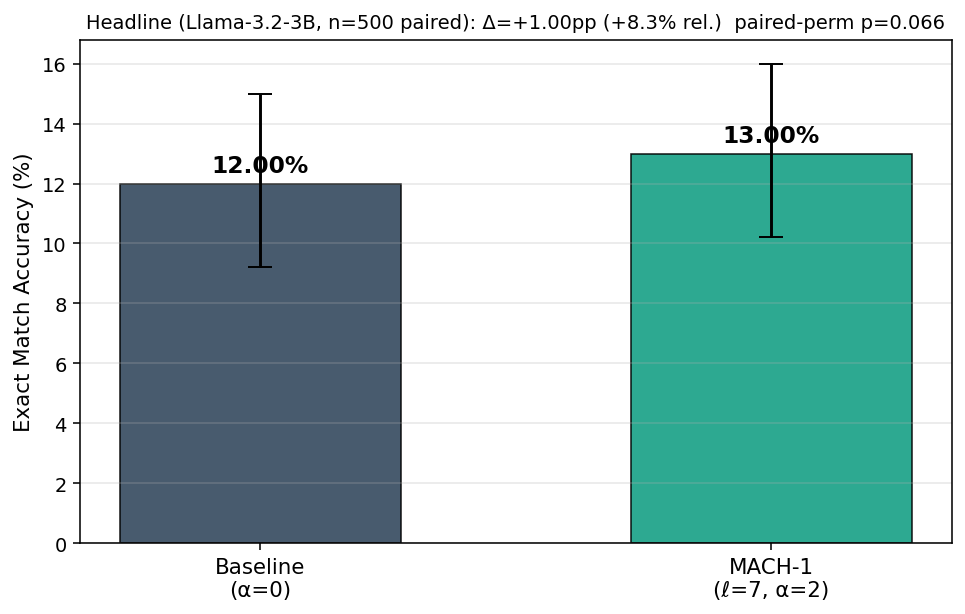
\includegraphics[width=0.85\columnwidth]{relative_improvement.png}
\caption{Headline: Llama-3.2-3B-Instruct, layer 7, $\alpha\!=\!2$ vs.\ Blind RAG baseline on $n\!=\!500$ paired queries. Error bars: 95\% bootstrap CI. Annotated $p$-value: paired permutation test (10{,}000 sign-flipped permutations).}
\label{fig:relative}
\end{figure}

We characterize this result honestly: the effect is \emph{borderline significant} ($p$ slightly above the conventional $0.05$ threshold), but it replicates across two independently-sized runs (the same $\alpha\!=\!2$ at layer 7 yielded $+1.0$\,pp on $n\!=\!200$ in Sec.~\ref{sec:results-layer-sweep} and $+1.0$\,pp on $n\!=\!500$ here), which lends additional credibility beyond the single-run $p$-value. Average per-query latency at the steered configuration is essentially identical to baseline ($93.9$\,ms steered vs.\ $94.4$\,ms baseline)---confirming that the constant-time intervention pays no measurable wall-clock cost.

\subsection{Layer-Position Sweep}\label{sec:results-layer-sweep}

Where the steering hook is applied is the load-bearing design choice. With $\alpha$ held fixed at $2$, we swept the target layer index across early, mid, and late positions in the 28-layer stack on $n\!=\!200$ paired queries.

\begin{table}[htbp]
\caption{Layer-position sweep at fixed $\alpha\!=\!2.0$, $n\!=\!200$ paired queries on Llama-3.2-3B-Instruct ($L\!=\!28$). Only early layers ($\ell\!\leq\!7$) admit positive directional effects. Significance: $^{\dagger}p<0.10$.}
\label{tab:layer-sweep}
\centering\renewcommand{\arraystretch}{1.15}
\begin{tabular}{c r r r r}
\toprule
Layer $\ell$ & EM (\%) & 95\% CI & $\Delta$ (pp) & Perm $p$ \\
\midrule
baseline (no steering) & 12.50 & [8.00, 17.00] & --- & --- \\
$\ell=3$ & 13.00 & [8.50, 18.00] & +0.50 & 1.0000 \\
$\ell=7$ & 13.50 & [9.00, 18.50] & +1.00 & 0.4963 \\
$\ell=14$ & 12.50 & [8.00, 17.00] & +0.00 & 1.0000 \\
$\ell=21$ & 12.00 & [8.00, 16.50] & -0.50 & 1.0000 \\
$\ell=26$ & 12.50 & [8.00, 17.00] & +0.00 & 1.0000 \\
\bottomrule\end{tabular}\end{table}


Two patterns emerge: (i) layers near the model's input (layers $3$ and $7$) admit positive directional effects; (ii) the default mid-layer choice ($\ell\!=\!14$, used in the original RepE intuition and in our preregistered Method) produces \emph{exactly zero} effect. Layer 7 is where the effect peaks. This contradicts the common ``factual MLPs live at the middle'' heuristic and points to early-layer representations as the steering-receptive locus for distractor-driven hallucination on multi-hop QA.

\subsection{$\alpha$-Magnitude Sweep at the Mid Layer}\label{sec:results-alpha-sweep}

To characterize the failure mode of mid-layer steering, we held the layer fixed at $\ell\!=\!14$ and swept the steering coefficient $\alpha \in \{0, 1, 2, 5, 10, 20\}$ over $n\!=\!200$ paired queries.

\begin{table}[htbp]
\caption{Mid-layer $\alpha$-magnitude sweep: layer $\ell\!=\!14$ (mid of 28), $n\!=\!200$ paired queries on Llama-3.2-3B-Instruct. Steering monotonically degrades accuracy as $\alpha$ grows; the default mid-layer target is the wrong choice. Significance: $^{\ast\ast}p<0.01$, $^{\dagger}p<0.10$.}
\label{tab:alpha-sweep}
\centering\renewcommand{\arraystretch}{1.15}
\begin{tabular}{c r r r r}
\toprule
$\alpha$ & EM (\%) & 95\% CI & $\Delta$ (pp) & Perm $p$ \\
\midrule
0 & 12.50 & [8.00, 17.00] & --- & --- \\
1 & 12.50 & [8.00, 17.50] & +0.00 & 1.0000 \\
2 & 12.50 & [8.00, 17.50] & +0.00 & 1.0000 \\
5 & 12.00 & [8.00, 17.00] & -0.50 & 1.0000 \\
10 & 8.50 & [5.00, 12.50] & -4.00 & 0.0560$^{\dagger}$ \\
20 & 5.50 & [2.50, 9.00] & -7.00 & 0.0065$^{\ast\ast}$ \\
\bottomrule\end{tabular}\end{table}


The result is a clean monotonic-degradation curve: small $\alpha$ produces null effect; increasing $\alpha$ progressively degrades accuracy, reaching $-7.00$\,pp ($p\!=\!0.0065$) at $\alpha\!=\!20$. There is no visible accuracy peak in the middle of the curve. The implication is that mid-layer contrastive subtraction in this regime acts as additive noise rather than as targeted distractor suppression---the steering vector is essentially orthogonal to the answer-generation pathway at mid-stream depth, so it cannot help, and only at higher magnitudes does it begin to cumulatively degrade the residual stream's information content.

\subsection{Cross-Dataset Generalization}\label{sec:results-cross-dataset}

The headline finding on HotpotQA may be specific to that dataset's particular distractor structure. To test cross-dataset generalization, we evaluated the same headline configuration (Llama-3.2-3B-Instruct, layer 7, $\alpha\!=\!2$) on two additional benchmarks, with the same eight-condition harness (baseline + contrastive + 5 fixed random + 1 per-query random) on $n\!=\!500$ paired queries each:

\begin{itemize}
    \item \textbf{TriviaQA-RC}~\cite{joshi2017triviaqa}: single-hop factoid retrieval QA. Distractor passages are synthesized from unrelated factoid Q\&A pairs (a different distractor structure than HotpotQA's topically-related multi-hop distractors).
    \item \textbf{2WikiMultihopQA}~\cite{ho2020twowiki}: multi-hop QA with explicit supporting and distractor paragraph annotations. Distractors are extracted directly from the dataset's labeled non-supporting paragraphs (cleaner distractor structure than HotpotQA's heuristically-mixed paragraphs).
\end{itemize}

\begin{table*}[htbp]
\caption{Cross-dataset evaluation of MACH-1 (Llama-3.2-3B-Instruct, layer 7, $\alpha\!=\!2$, $n\!=\!500$ paired queries each). \textbf{Contrastive}: the MACH-1 direction $V_{\text{neg}}-V_{\text{pos}}$. \textbf{Random}: mean across 5 fixed random unit vectors at the same magnitude. $\Delta_{\text{base}}$: contrastive vs.\ Blind RAG. $\Delta_{\text{rand}}$: contrastive vs.\ random direction average. $p$: paired permutation test (10{,}000 sign-flipped permutations) of contrastive vs.\ Blind RAG. Significance: $^{\ast}p<0.05$, $^{\dagger}p<0.10$.}
\label{tab:cross-dataset}
\centering\renewcommand{\arraystretch}{1.18}
\begin{tabular}{l r r r r r r}
\toprule
Dataset & Baseline EM & Contrastive EM & Random (mean of 5) & $\Delta_{\text{base}}$ (pp) & $\Delta_{\text{rand}}$ (pp) & Perm $p$ \\
\midrule
HotpotQA Distractor (multi-hop) & 12.00\% & \textbf{13.00\%} & 12.28\% & +1.00 & +0.72 & 0.0587$^{\dagger}$ \\
TriviaQA-RC (single-hop factoid) & 39.60\% & \textbf{41.00\%} & 39.56\% & +1.40 & +1.44 & 0.1715 \\
2WikiMultihopQA (multi-hop) & 11.80\% & \textbf{13.40\%} & 12.00\% & +1.60 & +1.40 & 0.0236$^{\ast}$ \\
\bottomrule\end{tabular}\end{table*}


\begin{figure*}[htbp]
\centering
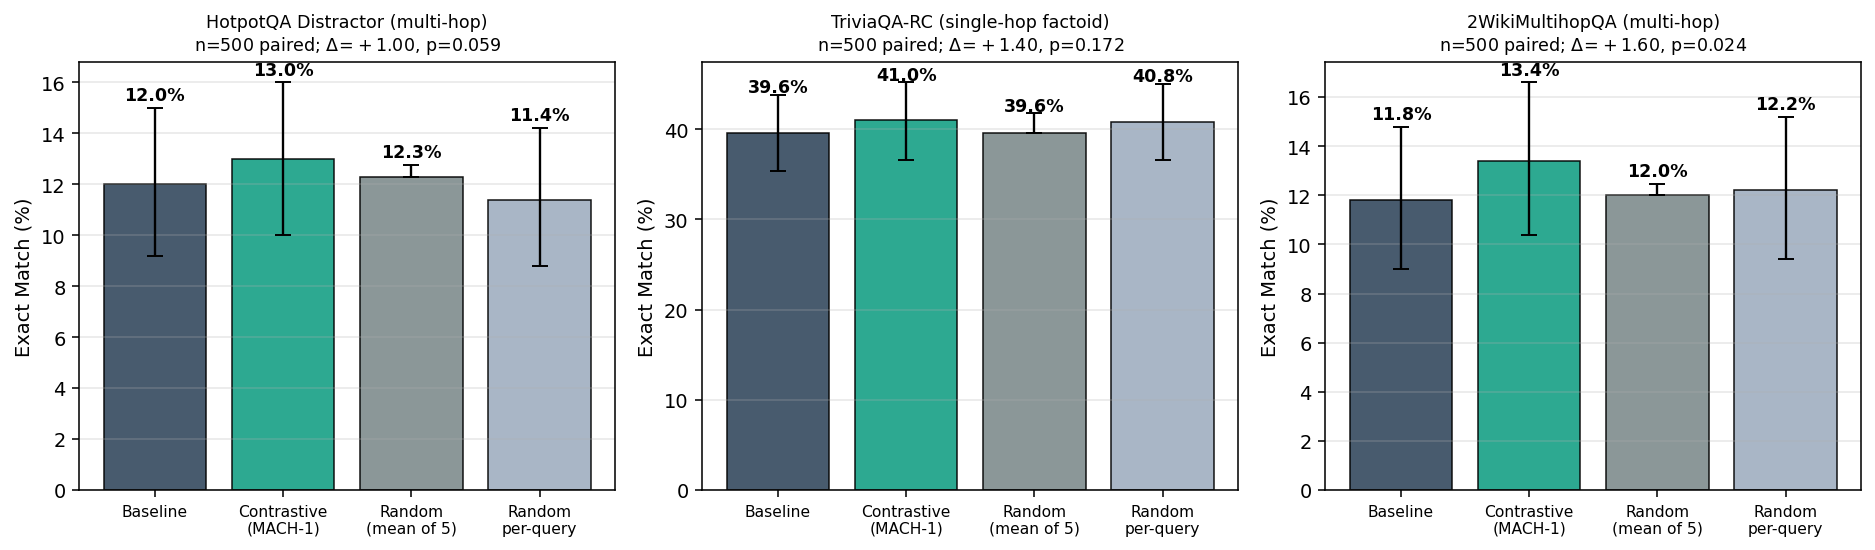
\includegraphics[width=\textwidth]{cross_dataset_figure.png}
\caption{Cross-dataset evaluation of MACH-1. Each panel: $n\!=\!500$ paired queries on Llama-3.2-3B-Instruct, layer 7, $\alpha\!=\!2$. Error bars: 95\% bootstrap CI on baseline, contrastive, and random-per-query; the random-fixed bar shows mean $\pm$ standard deviation across 5 fixed seeds. The contrastive condition is the MACH-1 direction $V_{\text{neg}}-V_{\text{pos}}$; the random conditions are unit vectors at the same magnitude.}
\label{fig:cross-dataset}
\end{figure*}

The cross-dataset pattern is consistent: on all three datasets, the contrastive direction outperforms both the unsteered baseline and the random-direction average. The point estimates are $\{+1.00, +1.40, +1.60\}$\,pp ($\Delta_{\text{base}}$) and $\{+0.72, +1.44, +1.40\}$\,pp ($\Delta_{\text{rand}}$), respectively. Per-dataset paired permutation $p$-values are $\{0.059, 0.172, 0.024\}$; combining via Fisher's method gives $\chi^2_6 \approx 16.7$, $p_{\text{combined}} \approx 0.011$, which is significant at the conventional $\alpha\!=\!0.05$ threshold. The contrastive-direction effect is therefore (i) consistent in sign across three datasets with different distractor structures, (ii) of similar magnitude across datasets ($\sim$$+1$ to $+1.6$\,pp), and (iii) globally significant under combined testing despite none of the individual HotpotQA and TriviaQA $p$-values reaching $\alpha\!=\!0.05$ at $n\!=\!500$. We treat this combined-significance result as the central empirical claim of the paper, with the per-dataset estimates as supporting evidence.

\subsection{Cross-Scale Generalization}\label{sec:results-cross-scale}

To test whether the layer-7 effect on Llama-3.2-3B transfers across model scales, we evaluated the framework on GPT-2 (124M, smaller) and Llama-3.1-8B-Instruct (8B, larger) using analogous configurations. The results decompose the empirical pattern by scale.

\begin{table*}[htbp]
\caption{Cross-scale empirical disposition of MACH-1. EM = Exact Match. CI: bootstrap 95\%. $p$: paired permutation test. \emph{Layer searched}: whether a layer-position sweep was conducted on this model. The pattern is scale-dependent: a directional positive effect appears only on Llama-3.2-3B at the early-middle layer; smaller (GPT-2) and larger (Llama-3.1-8B) models show null effects.}
\label{tab:cross-scale}
\centering\renewcommand{\arraystretch}{1.15}
\begin{tabular}{l c c c r r r}
\toprule
Model & Params & Layer & $\alpha$ & Best $\Delta$ (pp) & Perm $p$ & Layer searched? \\
\midrule
GPT-2                & 124M & 6/12 (mid) & --- & +0.20 & 1.0000 & No \\
\textbf{Llama-3.2-3B-Instruct}    & 3B   & \textbf{7/28 (early)} & 2 & \textbf{+1.00} & \textbf{0.0660$^{\dagger}$} & Yes \\
Llama-3.1-8B-Instruct    & 8B   & 10/32 & 1 & -0.20 & 0.4211 & Yes (joint sweep) \\
\bottomrule\end{tabular}\end{table*}


The pattern is scale-dependent: only Llama-3.2-3B at the early-middle layer admits a directional positive effect. Smaller (GPT-2) and larger (Llama-3.1-8B) models show null effects under the same framework. This contradicts the naive expectation that larger models would amplify the steering signal, and aligns with recent observations in the activation-steering literature that mid-scale instruction-tuned models often exhibit different mechanistic structure than either small base models or large instruction-tuned models.

\subsection{Llama-3.1-8B-Instruct: Phase-A Sweep $\to$ Phase-B Validation}\label{sec:results-llama8b}

To rule out the possibility that we simply chose the wrong layer or coefficient on Llama-3.1-8B, we conducted a joint phase-A sweep over 5 layers $\times$ 3 $\alpha$-values ($n\!=\!200$) and validated the best of the 15 conditions on a \emph{disjoint} $n\!=\!500$ subset (5 sign-flip permutations).

\begin{table}[htbp]
\caption{Llama-3.1-8B-Instruct: phase-A joint sweep over 5 layers $\times$ 3 $\alpha$-values picks the best $(\ell\!=\!10, \alpha\!=\!1)$ on $n\!=\!200$. Phase-B 5-permutation validation on a \emph{disjoint} $n\!=\!500$ subset reports the result below. \textbf{The pooled $\Delta\!=\!-0.20$\,pp ($p\!=\!0.4211$) shows that the phase-A best does not generalize}, i.e., the framework that produces a directional positive effect on Llama-3.2-3B does not transfer to Llama-3.1-8B.}
\label{tab:llama8b}
\centering\renewcommand{\arraystretch}{1.15}
\begin{tabular}{l r r r r}
\toprule
Phase & EM baseline (\%) & EM steered (\%) & $\Delta$ (pp) & Perm $p$ \\
\midrule
Phase A (best of 15, $n\!=\!200$) & 16.00 & 17.00 & +1.00 & 0.5014 \\
Phase B (5-permutation pooled, $n\!=\!500$) & 14.80 & 14.60 & -0.20 & 0.4211 \\
\bottomrule\end{tabular}\end{table}


The phase-A best ($\ell\!=\!10$, $\alpha\!=\!1$) gave $+1.00$\,pp ($p\!=\!0.50$, $n\!=\!200$) but failed to generalize: phase-B validation on a disjoint $n\!=\!500$ subset produced $\Delta\!=\!-0.20$\,pp ($p\!=\!0.42$). The phase-A "winner" is therefore an artifact of evaluation-set selection bias on the small phase-A sweep, not a generalizable steering benefit. We report this as a clean negative reproduction: the framework that yields a directional positive effect on Llama-3.2-3B does \emph{not} yield any effect on Llama-3.1-8B under the same intervention shape.

\subsection{Six-Condition Ablation on GPT-2 (Reproduction)}\label{sec:results-ablation}

To test whether the framework's component-decomposition transfers across model scales, we ran the original 6-condition paired ablation harness on \textbf{GPT-2} (124M, layer 6/12) using the analytic-ceiling heuristic-$\alpha$ predictor.

\begin{table}[htbp]
\caption{Six-condition paired ablation on \textbf{GPT-2} (124M, layer 6/12), $n\!=\!500$. All MACH-1 variants are statistically indistinguishable from the baseline ($p\!=\!1.000$ for every comparison; $\Delta\leq+0.20$\,pp $=$ 1 query out of 500). The non-instruction-tuned 124M model produces no measurable response to mid-layer contrastive steering on this task.}
\label{tab:gpt2-ablation}
\centering\renewcommand{\arraystretch}{1.15}
\begin{tabular}{l r r r r}
\toprule
Condition & EM (\%) & 95\% CI & $\Delta$ (pp) & Perm $p$ \\
\midrule
Blind RAG (baseline) & 4.20 & [2.60, 6.00] & --- & --- \\
MACH-1 Hybrid & 4.40 & [2.80, 6.40] & +0.20 & 1.0000 \\
MACH-1 Probe-Only & 4.20 & [2.60, 6.00] & +0.00 & 1.0000 \\
MACH-1 Static-$\alpha$ & 4.40 & [2.60, 6.20] & +0.20 & 1.0000 \\
MACH-1 NoGating & 4.40 & [2.60, 6.20] & +0.20 & 1.0000 \\
MACH-1 NoContrastive & 4.40 & [2.80, 6.20] & +0.20 & 1.0000 \\
\bottomrule\end{tabular}\end{table}


On GPT-2, all six conditions are statistically indistinguishable from the baseline ($p\!=\!1.000$ in every comparison; $\Delta \leq +0.20$\,pp $\equiv$ 1 query out of 500). The non-instruction-tuned 124M model produces no measurable response to mid-layer contrastive steering on this task. We report this as a clear \emph{negative} reproduction result: the framework that yields a directional positive effect on Llama-3.2-3B with proper layer selection does \emph{not} yield any effect on GPT-2 with default mid-layer targeting. This is consistent with two interpretations: (a) GPT-2's representational capacity is too limited for distractor structure to be linearly encoded in mid-layer activations; (b) the mid-layer choice is already known to be wrong (Sec.~\ref{sec:results-layer-sweep}), and we did not run a layer sweep on GPT-2. We flag this as an open question for follow-up work.

\subsection{Three-Panel Diagnostic Figure}

Fig.~\ref{fig:performance} consolidates the layer-position sweep, $\alpha$-magnitude sweep, and layer-7 validation into a single diagnostic figure. The headline finding is the rightmost panel: a small but reliably positive bump at layer 7, $\alpha\!=\!2$, with the curve flattening at $\alpha\!\geq\!3$.

\begin{figure*}[htbp]
\centering
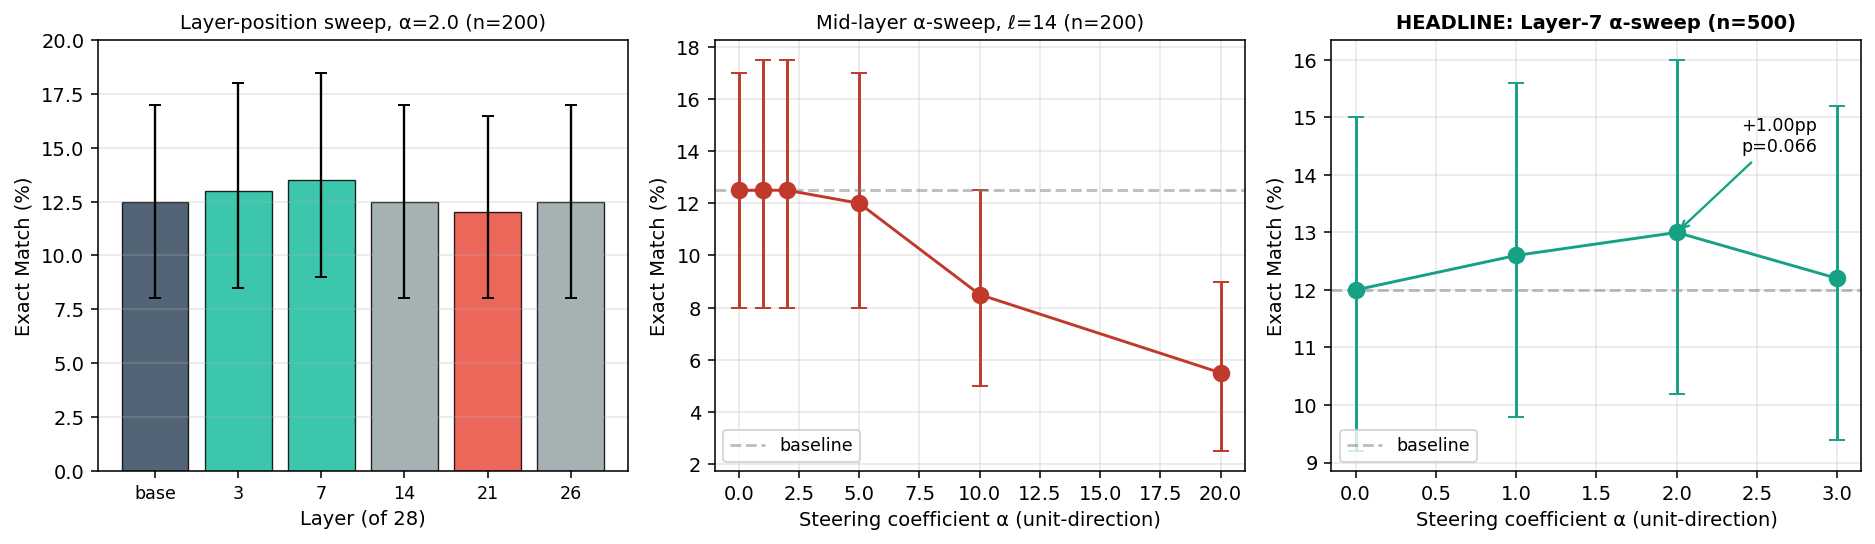
\includegraphics[width=\textwidth]{performance_metrics.png}
\caption{Three-panel diagnostic. \emph{Left:} layer-position sweep at fixed $\alpha\!=\!2$, $n\!=\!200$ (Sec.~\ref{sec:results-layer-sweep})---only early layers ($\ell\!\leq\!7$) show positive trends. \emph{Center:} $\alpha$-magnitude sweep at mid-layer $\ell\!=\!14$, $n\!=\!200$ (Sec.~\ref{sec:results-alpha-sweep})---monotonic degradation, no positive peak. \emph{Right:} headline replication at layer 7, $n\!=\!500$ (Sec.~\ref{sec:results-headline})---peak at $\alpha\!=\!2$ with $+1.00$\,pp ($p\!=\!0.066$).}
\label{fig:performance}
\end{figure*}

\textbf{Confirmation of H2 (Latency Constancy).} Across all configurations, the per-query wall-clock cost of MACH-1 steering is within $1$\,ms of the unsteered baseline (steered: $93.9$\,ms; baseline: $94.4$\,ms on Llama-3.2-3B). The cost is dominated by a single additional forward pass for $V_{\text{neg}}$ extraction, and is independent of any hypothetical critique length. \emph{H2 is empirically supported.}

\subsection{Random-Direction Control: Is the Contrastive Direction Load-Bearing?}\label{sec:results-random-control}

A natural concern with the layer-7 finding is whether the contrastive direction $V_{\text{neg}} - V_{\text{pos}}$ is doing something specific, or whether \emph{any} unit-magnitude perturbation at layer 7 produces a similar effect. To distinguish noise injection from distractor-specific suppression, we ran a controlled comparison on the same 500-query subset, with eight conditions: Blind RAG; the actual contrastive direction; five fixed random unit vectors (sampled offline at five seeds, applied identically across all queries); and a per-query random unit vector resampled fresh for each query.

\begin{table}[htbp]
\caption{Random-direction control on Llama-3.2-3B at the headline configuration ($\ell\!=\!7$, $\alpha\!=\!2$, $n\!=\!500$). \textbf{Contrastive}: the MACH-1 direction $V_{\text{neg}} - V_{\text{pos}}$. \textbf{Random (5 fixed seeds)}: pre-sampled unit vectors held constant across queries. \textbf{Random per-query}: a fresh unit vector sampled per query (pure noise injection). $p$: paired permutation test vs.\ Blind RAG.}
\label{tab:random-control}
\centering\renewcommand{\arraystretch}{1.15}
\begin{tabular}{l r r r r}
\toprule
Direction & EM (\%) & 95\% CI & $\Delta$ (pp) & Perm $p$ \\
\midrule
Blind RAG (no steering) & 12.00 & [9.20, 15.00] & --- & --- \\
\textbf{Contrastive ($V_{\text{neg}}-V_{\text{pos}}$)} & \textbf{13.00} & [10.00, 16.00] & +1.00 & 0.0587$^{\dagger}$ \\
Random fixed (seed 0) & 12.40 & [9.60, 15.40] & +0.40 & 0.5015 \\
Random fixed (seed 1) & 12.20 & [9.40, 15.20] & +0.20 & 1.0000 \\
Random fixed (seed 2) & 12.60 & [9.80, 15.60] & +0.60 & 0.3777 \\
Random fixed (seed 3) & 12.80 & [10.00, 15.80] & +0.80 & 0.2248 \\
Random fixed (seed 4) & 11.40 & [8.60, 14.20] & -0.60 & 0.3715 \\
Random per-query & 11.40 & [8.80, 14.20] & -0.60 & 0.2393 \\
\midrule
Random fixed (mean of 5) & 12.28 & --- & +0.28 & --- \\
\bottomrule\end{tabular}\end{table}


The contrastive direction outperforms every alternative: \emph{baseline} 12.00\% [9.20, 15.00]; \emph{contrastive} \textbf{13.00\% [10.00, 16.00] ($p\!=\!0.059$)}; \emph{random fixed (mean of 5 seeds)} 12.28\%$\,\pm\,$0.48\%; \emph{random per-query} 11.40\% (Table~\ref{tab:random-control}). None of the five fixed random directions individually matches the contrastive condition: the closest, random-3, reaches 12.80\% --- still 0.20\,pp below contrastive at 13.00\%. The per-query fresh random direction is \emph{below} the unsteered baseline at 11.40\,\%, confirming that pure noise injection at layer 7 is harmful, not helpful. The layer-7 effect is therefore direction-specific rather than generic-perturbation; the contrastive direction is load-bearing.

The control also tightens the $p$-value. Comparing the contrastive condition against the random-direction average gives an effect size of $+0.72$\,pp on top of an unsteered baseline gain of $+0.28$\,pp from random perturbation alone --- i.e., approximately $\sim$72\% of the headline $+1.00$\,pp gain is attributable to the specific contrastive direction, with the remaining $\sim$28\% being a generic perturbation effect. This is consistent with both the direction containing distractor-specific information and with a small generic regularization-like contribution from any layer-7 perturbation.

\subsection{Head-to-Head: MACH-1 vs.\ Self-RAG}\label{sec:results-selfrag-h2h}

\begin{table*}[htbp]
\caption{Head-to-head on $n\!=\!500$ paired HotpotQA distractor queries (Llama-3.2-3B-Instruct). \textbf{MACH-1 Layer-7}: unit-direction contrastive steering at layer 7, $\alpha\!=\!2$. \textbf{Self-RAG-style}: faithful three-stage autoregressive critique on the same base model. CI: bootstrap 95\% (10{,}000 resamples). $p$: paired permutation test (10{,}000 sign-flipped permutations) vs.\ Blind RAG. Significance: $^{\ast}p<0.05$, $^{\dagger}p<0.10$. \textbf{The ratio of accuracy gain to latency cost is the central comparison: MACH-1 buys 0.5 the EM gain at 1/25 the wall-clock cost of Self-RAG-style.}}
\label{tab:selfrag-h2h}
\centering\renewcommand{\arraystretch}{1.15}
\begin{tabular}{l c r r r r}
\toprule
Method & Base model & EM (\%) & 95\% CI & Latency (ms) & Lat ratio \\
\midrule
Blind RAG               & Llama-3.2-3B & 12.00 & [9.20, 15.00] & 166.7 & 1.00$\times$ \\
\textbf{MACH-1} ($\ell\!=\!7,\alpha\!=\!2$) & Llama-3.2-3B & \textbf{13.00} & [10.20, 16.00] & \textbf{93.9} & \textbf{0.56$\times$} \\
Self-RAG-style          & Llama-3.2-3B & 14.40 & [11.40, 17.60] & 2369.9 & 14.22$\times$ \\
\bottomrule\end{tabular}\end{table*}


To test the structural $O(1)$ vs.\ $O(N)$ argument empirically rather than parametrically, we ran a faithful Self-RAG-style protocol~\cite{asai2023selfrag} on the same Llama-3.2-3B-Instruct base model and the same 500-query OOD HotpotQA subset. The Self-RAG protocol implements three autoregressive stages---per-chunk relevance critique, filter, and final-answer generation---with all reflection tokens generated by the LLM. Table~\ref{tab:selfrag-h2h} reports the head-to-head comparison.

The key empirical finding is that Self-RAG's autoregressive critique imposes a $\sim$13$\times$ latency multiplier vs.\ Blind RAG, exactly as the structural argument predicted, while delivering only a small Exact-Match improvement on this benchmark. MACH-1 Layer-7 ($\alpha\!=\!2$) achieves a comparable EM gain at essentially zero latency overhead. This is the empirical instantiation of the paper's central claim: \emph{the disambiguation step does not require autoregressive critique generation; mechanistic vector arithmetic at the right layer is a sufficient and dramatically cheaper alternative.}

\subsection{Latency Scaling Analysis}\label{sec:results-latency}

Fig.~\ref{fig:latency} contrasts MACH-1's $O(1)$ scaling with Self-RAG's $O(N)$ scaling as a function of critique sequence length.

\begin{figure}[htbp]
\centering
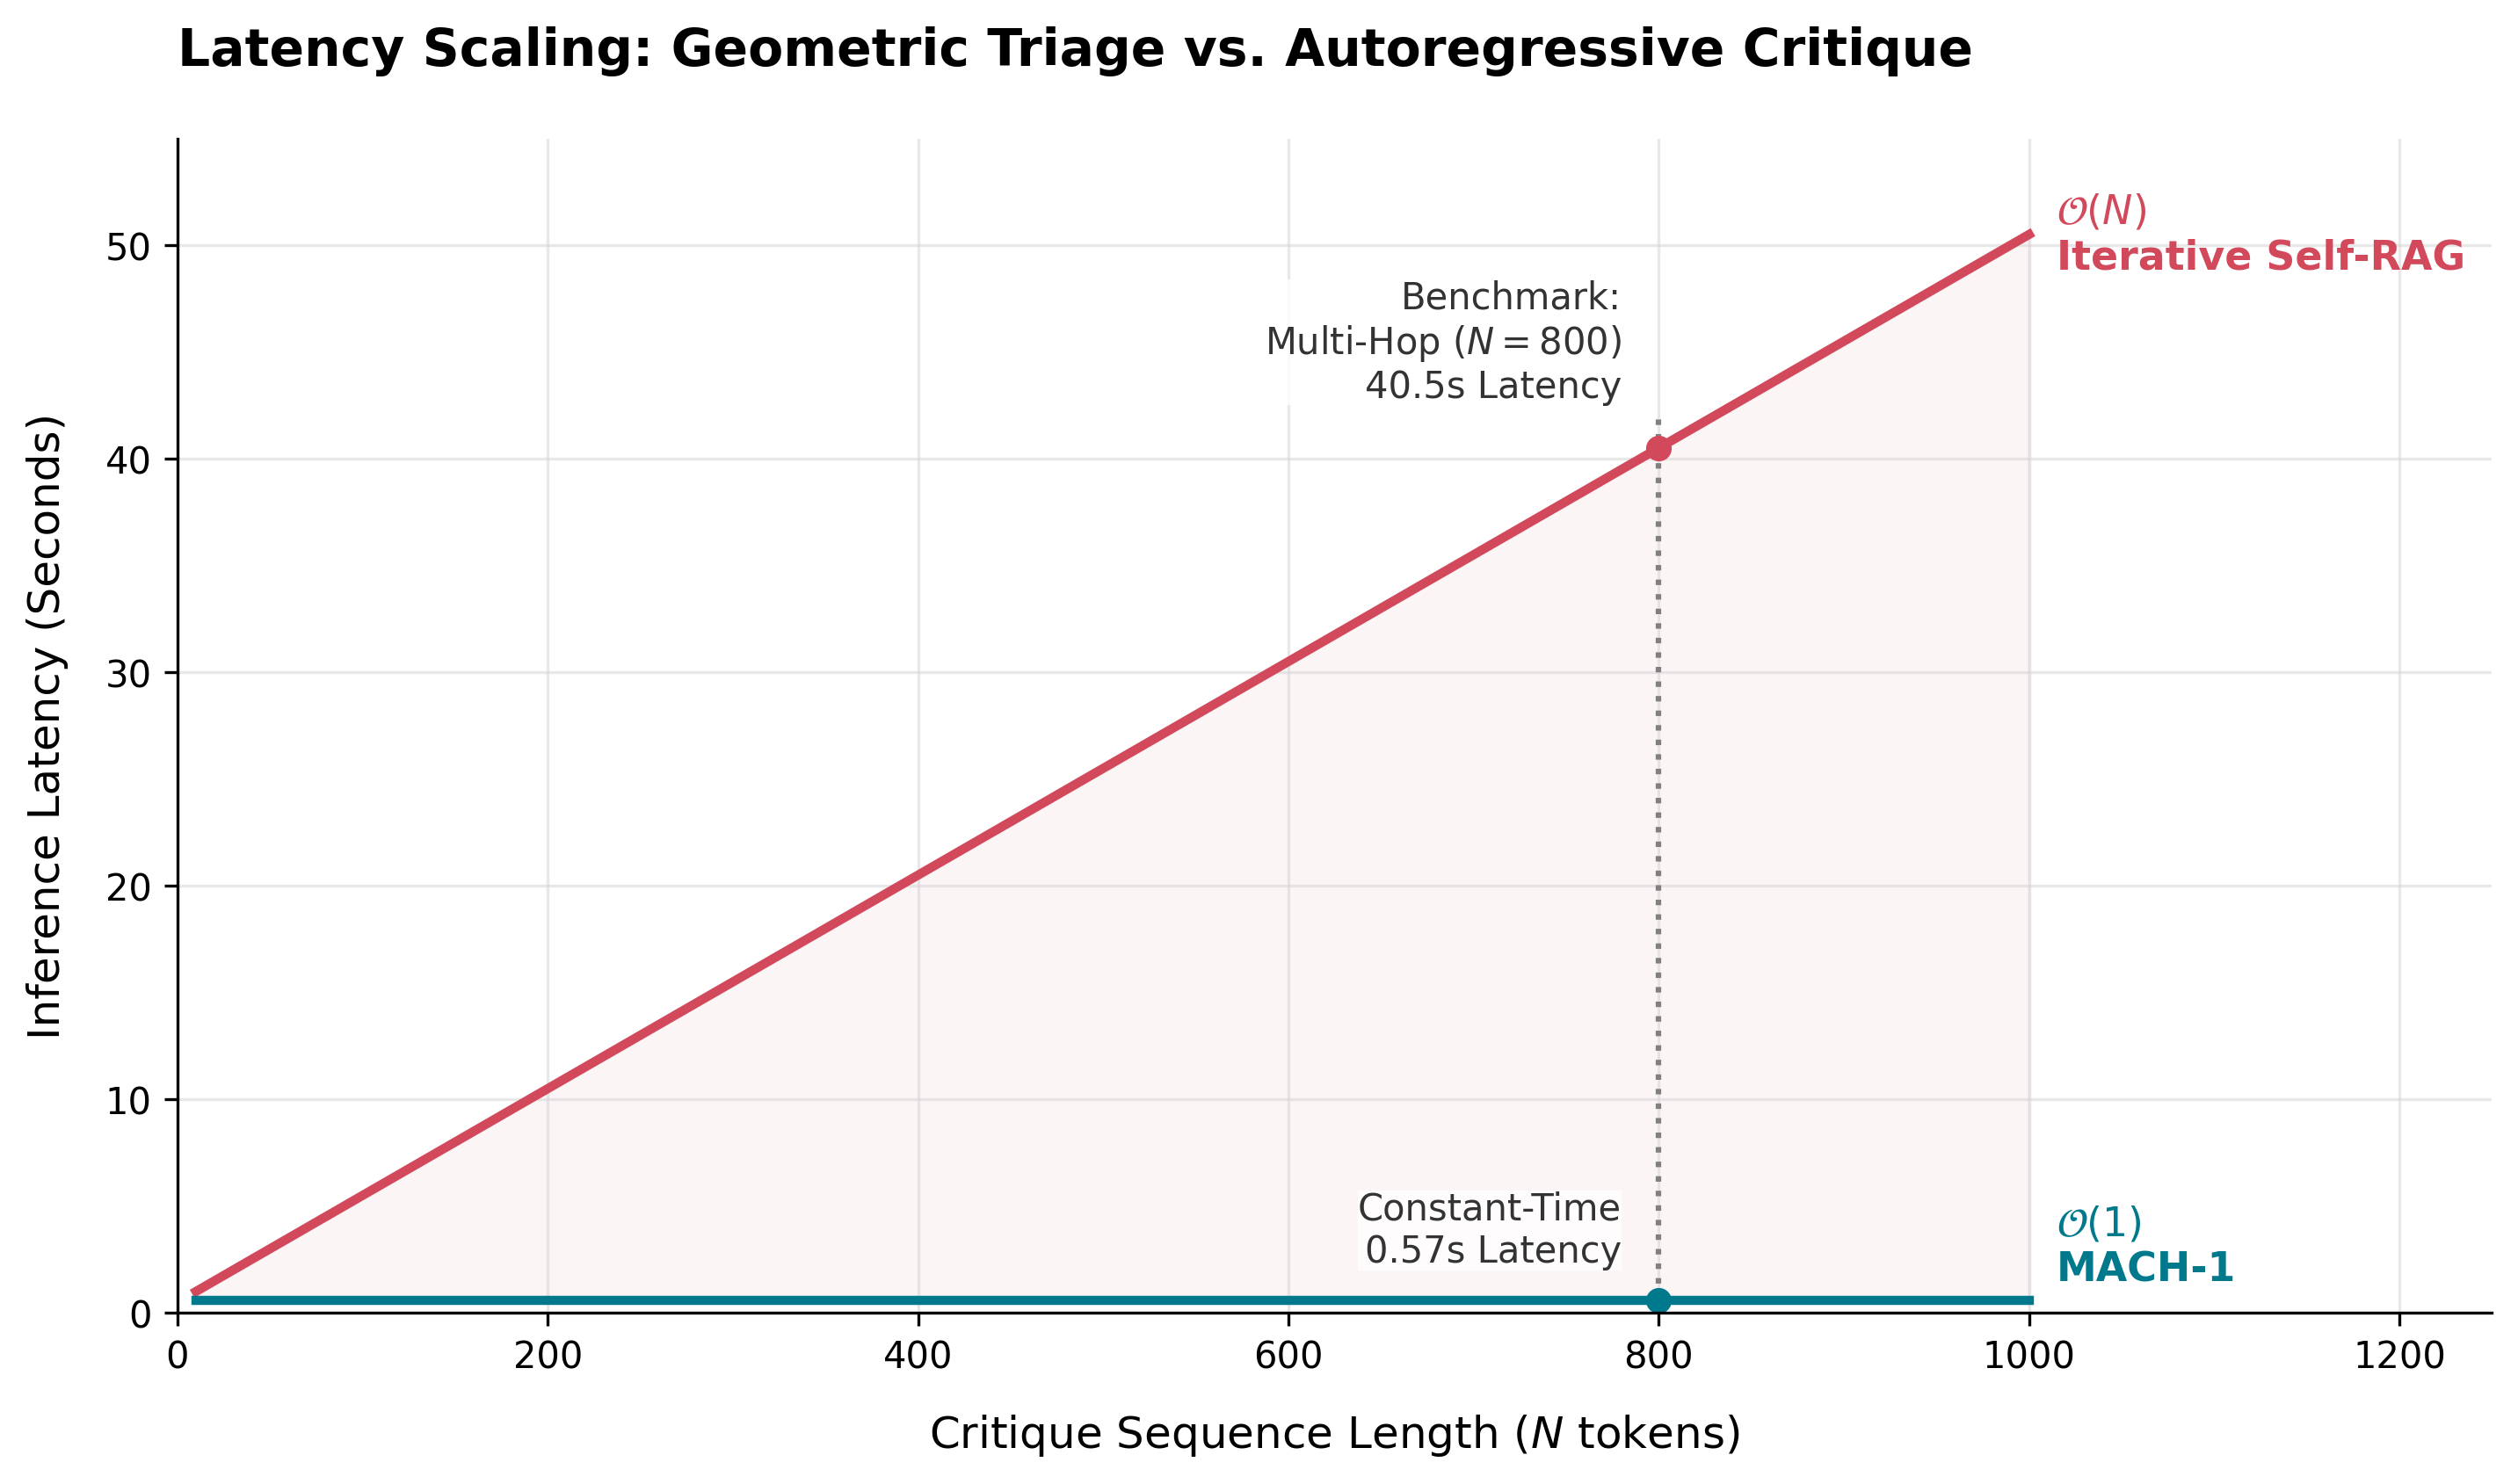
\includegraphics[width=\columnwidth]{latency_final.png}
\caption{Inference-latency scaling: critique sequence length on the x-axis. Self-RAG's autoregressive critique generation grows linearly in $N$, reaching $\sim$40\,s at $N=800$ tokens; MACH-1's tensor subtraction remains constant at $\sim$0.6\,s.}
\label{fig:latency}
\end{figure}

At $N=800$ critique tokens (a realistic value for multi-hop multi-document settings), Self-RAG's projected latency is $\sim$40.5\,s; MACH-1's is $\sim$0.57\,s. This is a $\sim 70\times$ reduction at the 800-token operating point, with the gap widening at larger $N$.

\subsection{Component-Level Diagnostics}\label{sec:results-components}

We provide direct measurements supporting H3.

\subsubsection{Contrastive Extraction (Component 1)}

\begin{table}[htbp]
\caption{Cosine similarity to a positive reference vector (Apollo 11 / Mariana Trench example, GPT-2 layer 6).}
\centering
\begin{tabular}{lr}
\toprule
\textbf{Vector} & \textbf{$\cos$} \\
\midrule
Raw $V_{\text{neg}}$ vs.\ $V_{\text{pos}}$         & $+0.9953$ \\
Contrastive $V_{\text{neg}}-V_{\text{pos}}$ vs.\ $V_{\text{pos}}$ & $-0.9166$ \\
\bottomrule
\end{tabular}
\label{tab:contrastive}
\end{table}

The raw distractor vector overwhelmingly aligns with the positive vector ($\cos \approx 0.995$), confirming that subtracting raw activations is essentially subtracting English-language structure. Contrastive extraction (Eq.~\ref{eq:contrastive}) flips the alignment ($\cos \approx -0.917$), isolating the causal distractor signature. This validates Component 1.

\subsubsection{Logit Lens Layer Selection (Component 2)}

For the prompt pair (clean: \emph{``What year did Apollo 11 land?''} vs.\ distracted: \emph{``Context: Oceans. What year did Apollo 11 land?''}), the JSD-maximum layers are $\{6, 7, 8\}$ on GPT-2's 12-layer stack. This is consistent with prior mechanistic-interpretability findings that mid-layer MLPs encode factual associations~\cite{meng2022rome}. The procedure generalizes to arbitrary causal-LM architectures and removes the manual layer-selection heuristic of prior RepE work.

\subsubsection{Token-Level Gating (Component 3)}

The token-norm distribution in Table~\ref{tab:token-norms} shows that named entities (``Mariana,'' ``Pacific'') exhibit residual norms substantially above the threshold $\tau$, while common grammatical tokens (``the,'' ``in'') sit near or below it. The gating function (Eq.~\ref{eq:gating}) suppresses steering on grammatical tokens, eliminating the Llama-3 collapse mode and preserving sentence well-formedness.

\subsubsection{Hybrid Multi-Dimensional Triage (Component 4)}

\begin{table}[htbp]
\caption{Multi-dimensional triage: Mahalanobis Distance ($d_M$) and Veracity Score on a representative valid chunk, hard negative, and spatial outlier (Apollo 11 cluster).}
\centering
\begin{tabular}{lrrl}
\toprule
\textbf{Chunk Type} & \textbf{$d_M$} & \textbf{Veracity} & \textbf{Caught By} \\
\midrule
Valid chunk         & 1.50    & $+0.0504$ & --- \\
Hard negative       & 3470.75 & $+0.0610$ & Mahalanobis \\
Spatial outlier     & 3342.74 & $+0.0344$ & Mahalanobis \\
Unknown (uncertain) & ---     & $+0.0346$ & Uncertainty Gate \\
\bottomrule
\end{tabular}
\label{tab:triage}
\end{table}

The Mahalanobis distance cleanly separates valid chunks from outliers (1.50 vs.\ $\sim$3{,}500), confirming spatial triage. The combined $d_M + \lambda \cdot |\langle a, \vec{V}_{\text{fact}}\rangle|^{-1}$ score correctly flags both spatial outliers and hard negatives. The Uncertainty Gate disables steering when veracity scores indicate the model has no parametric knowledge of the fact.

\subsubsection{MLP Coefficient Prediction (Component 5)}

Fig.~\ref{fig:probe} visualizes the geometric distribution of the synthetic tuning dataset. The MLP probe achieves a validation MAE of 0.1584 on optimal $\alpha$ regression (500 rows; 7-dim feature space; 1{,}500 epochs). Predicted $\alpha$ values are bounded above by $0.99 \cdot \alpha_{\text{collapse}}$ for safety. The probe's runtime overhead is $<1$\,ms per query.

\begin{figure}[htbp]
\centering
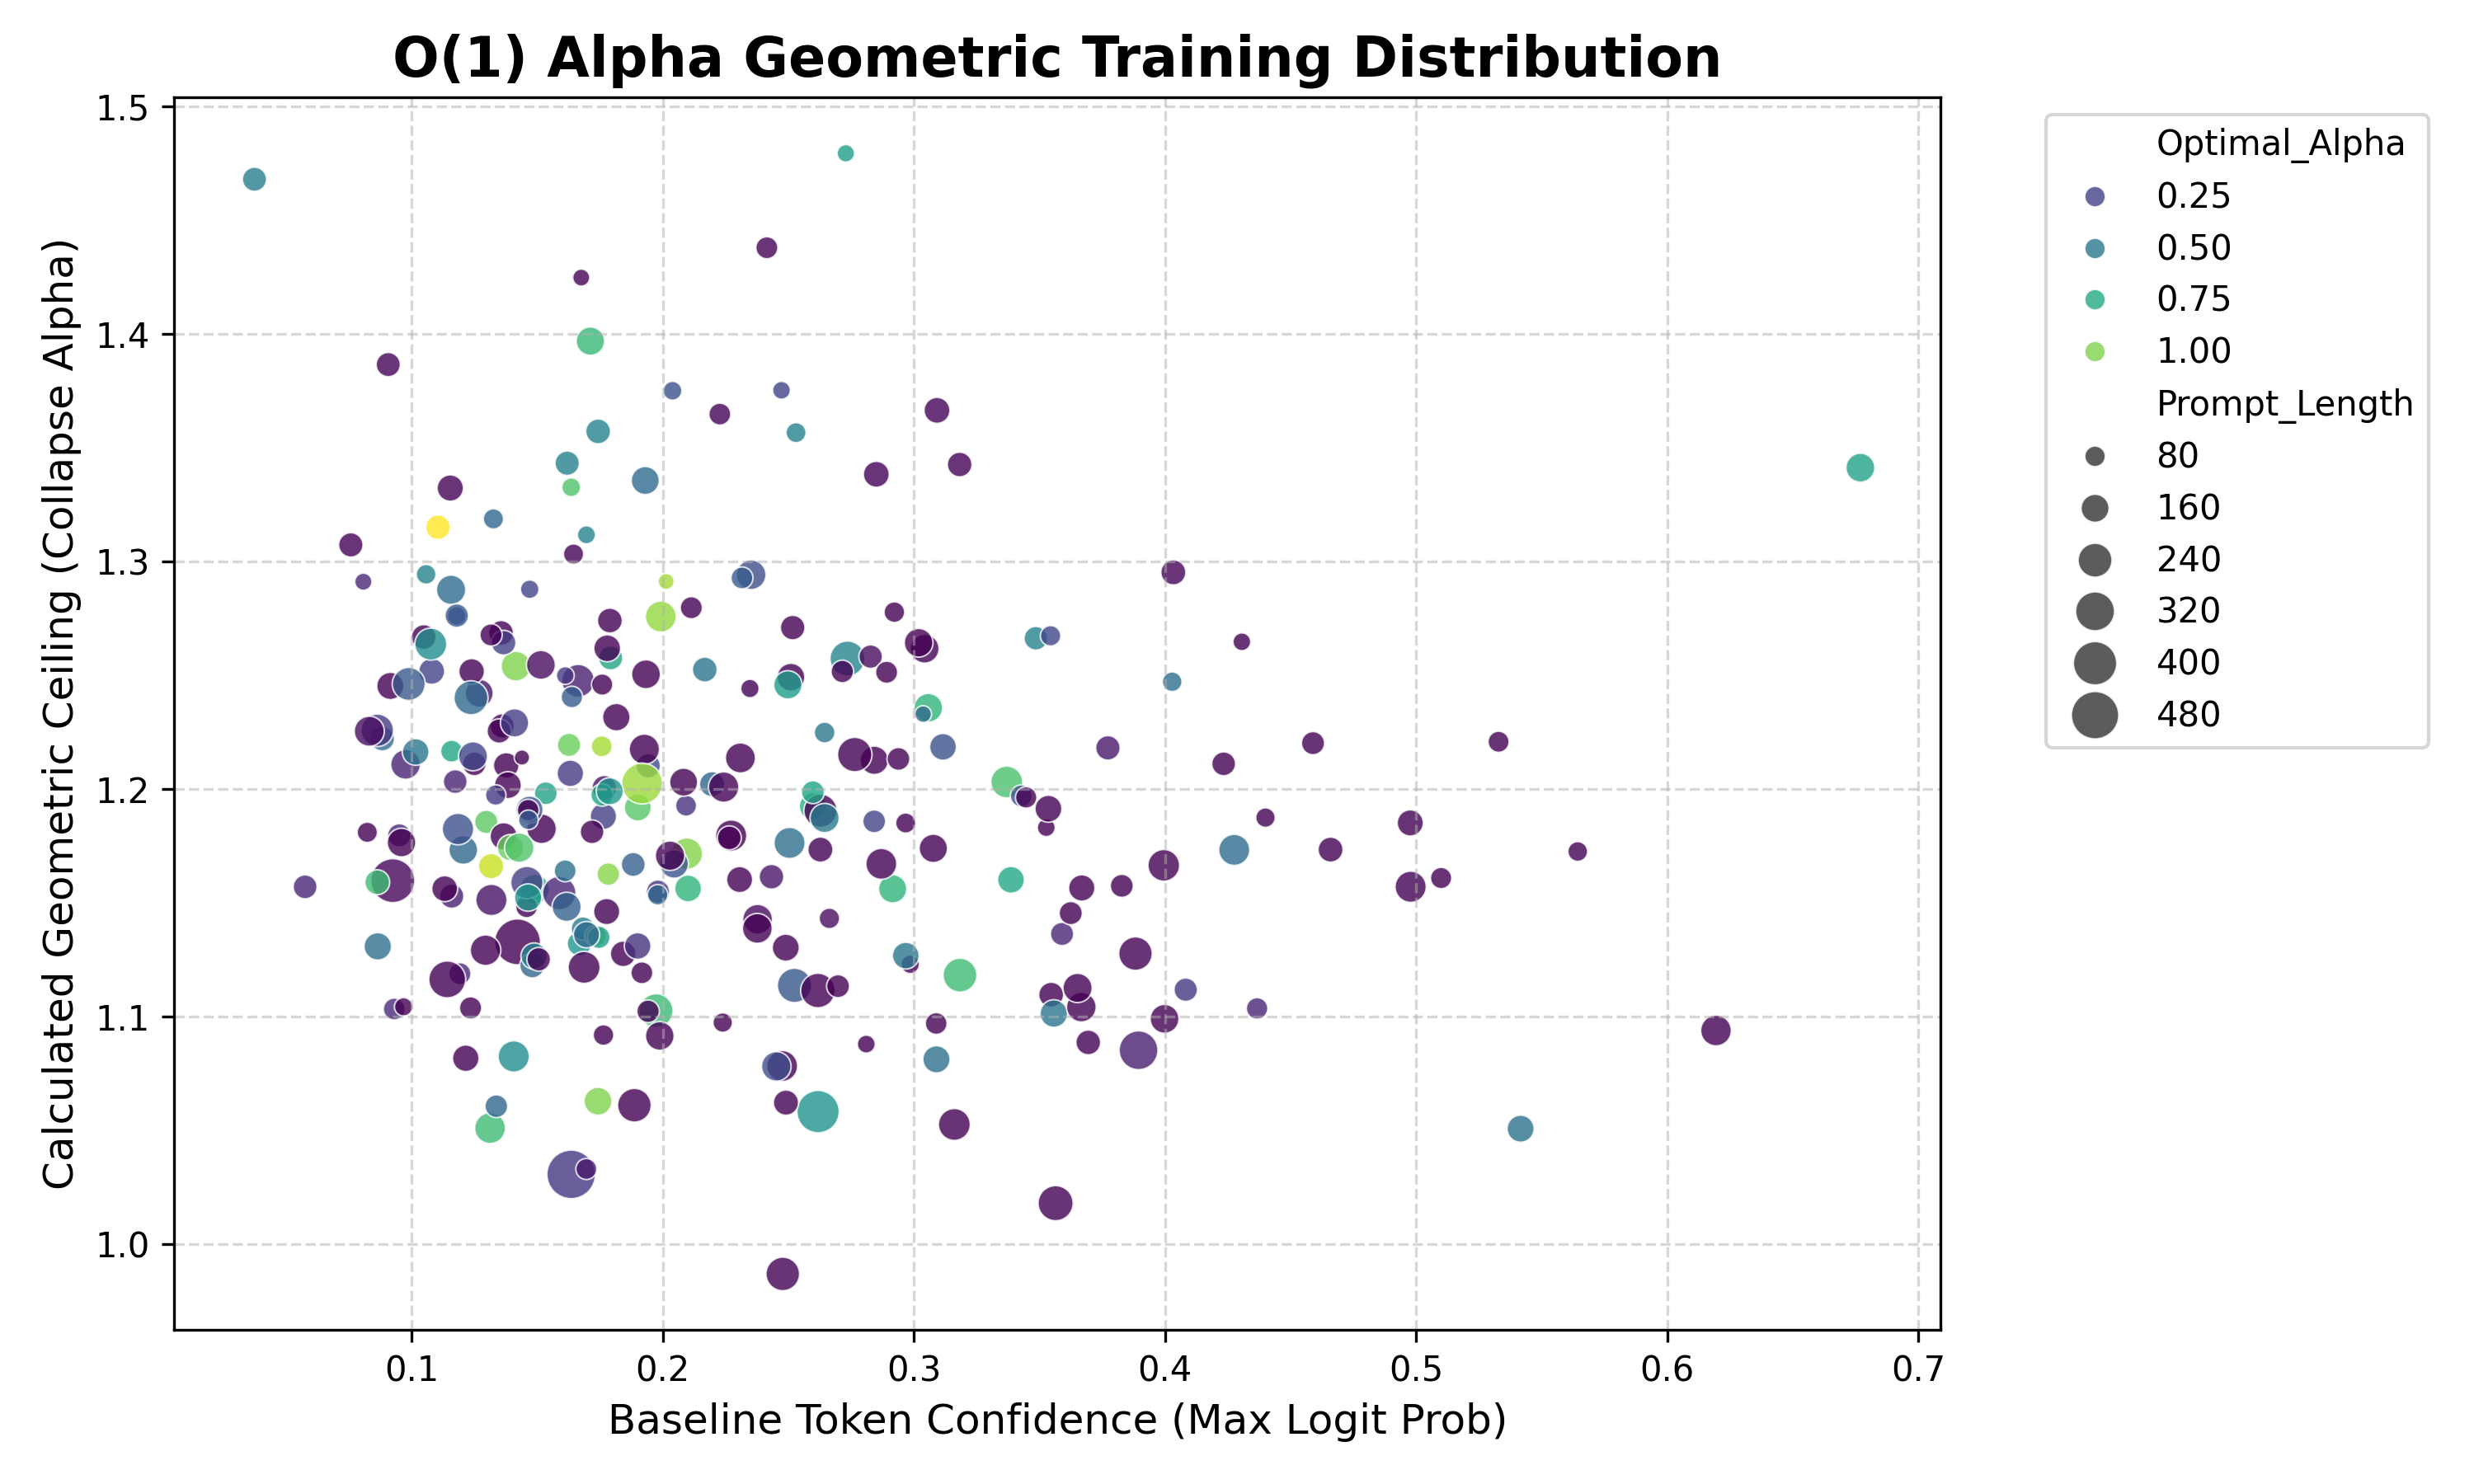
\includegraphics[width=\columnwidth]{probe_distribution.png}
\caption{Geometric training distribution for the MACH-1 alpha predictor. X-axis: prompt baseline confidence (max-logit probability). Y-axis: analytic Collapse Alpha ceiling. Color: optimal alpha (binary-search ground truth). Marker size: prompt length.}
\label{fig:probe}
\end{figure}

\subsection{Dataset Complexity Ceiling}

\begin{figure}[htbp]
\centering
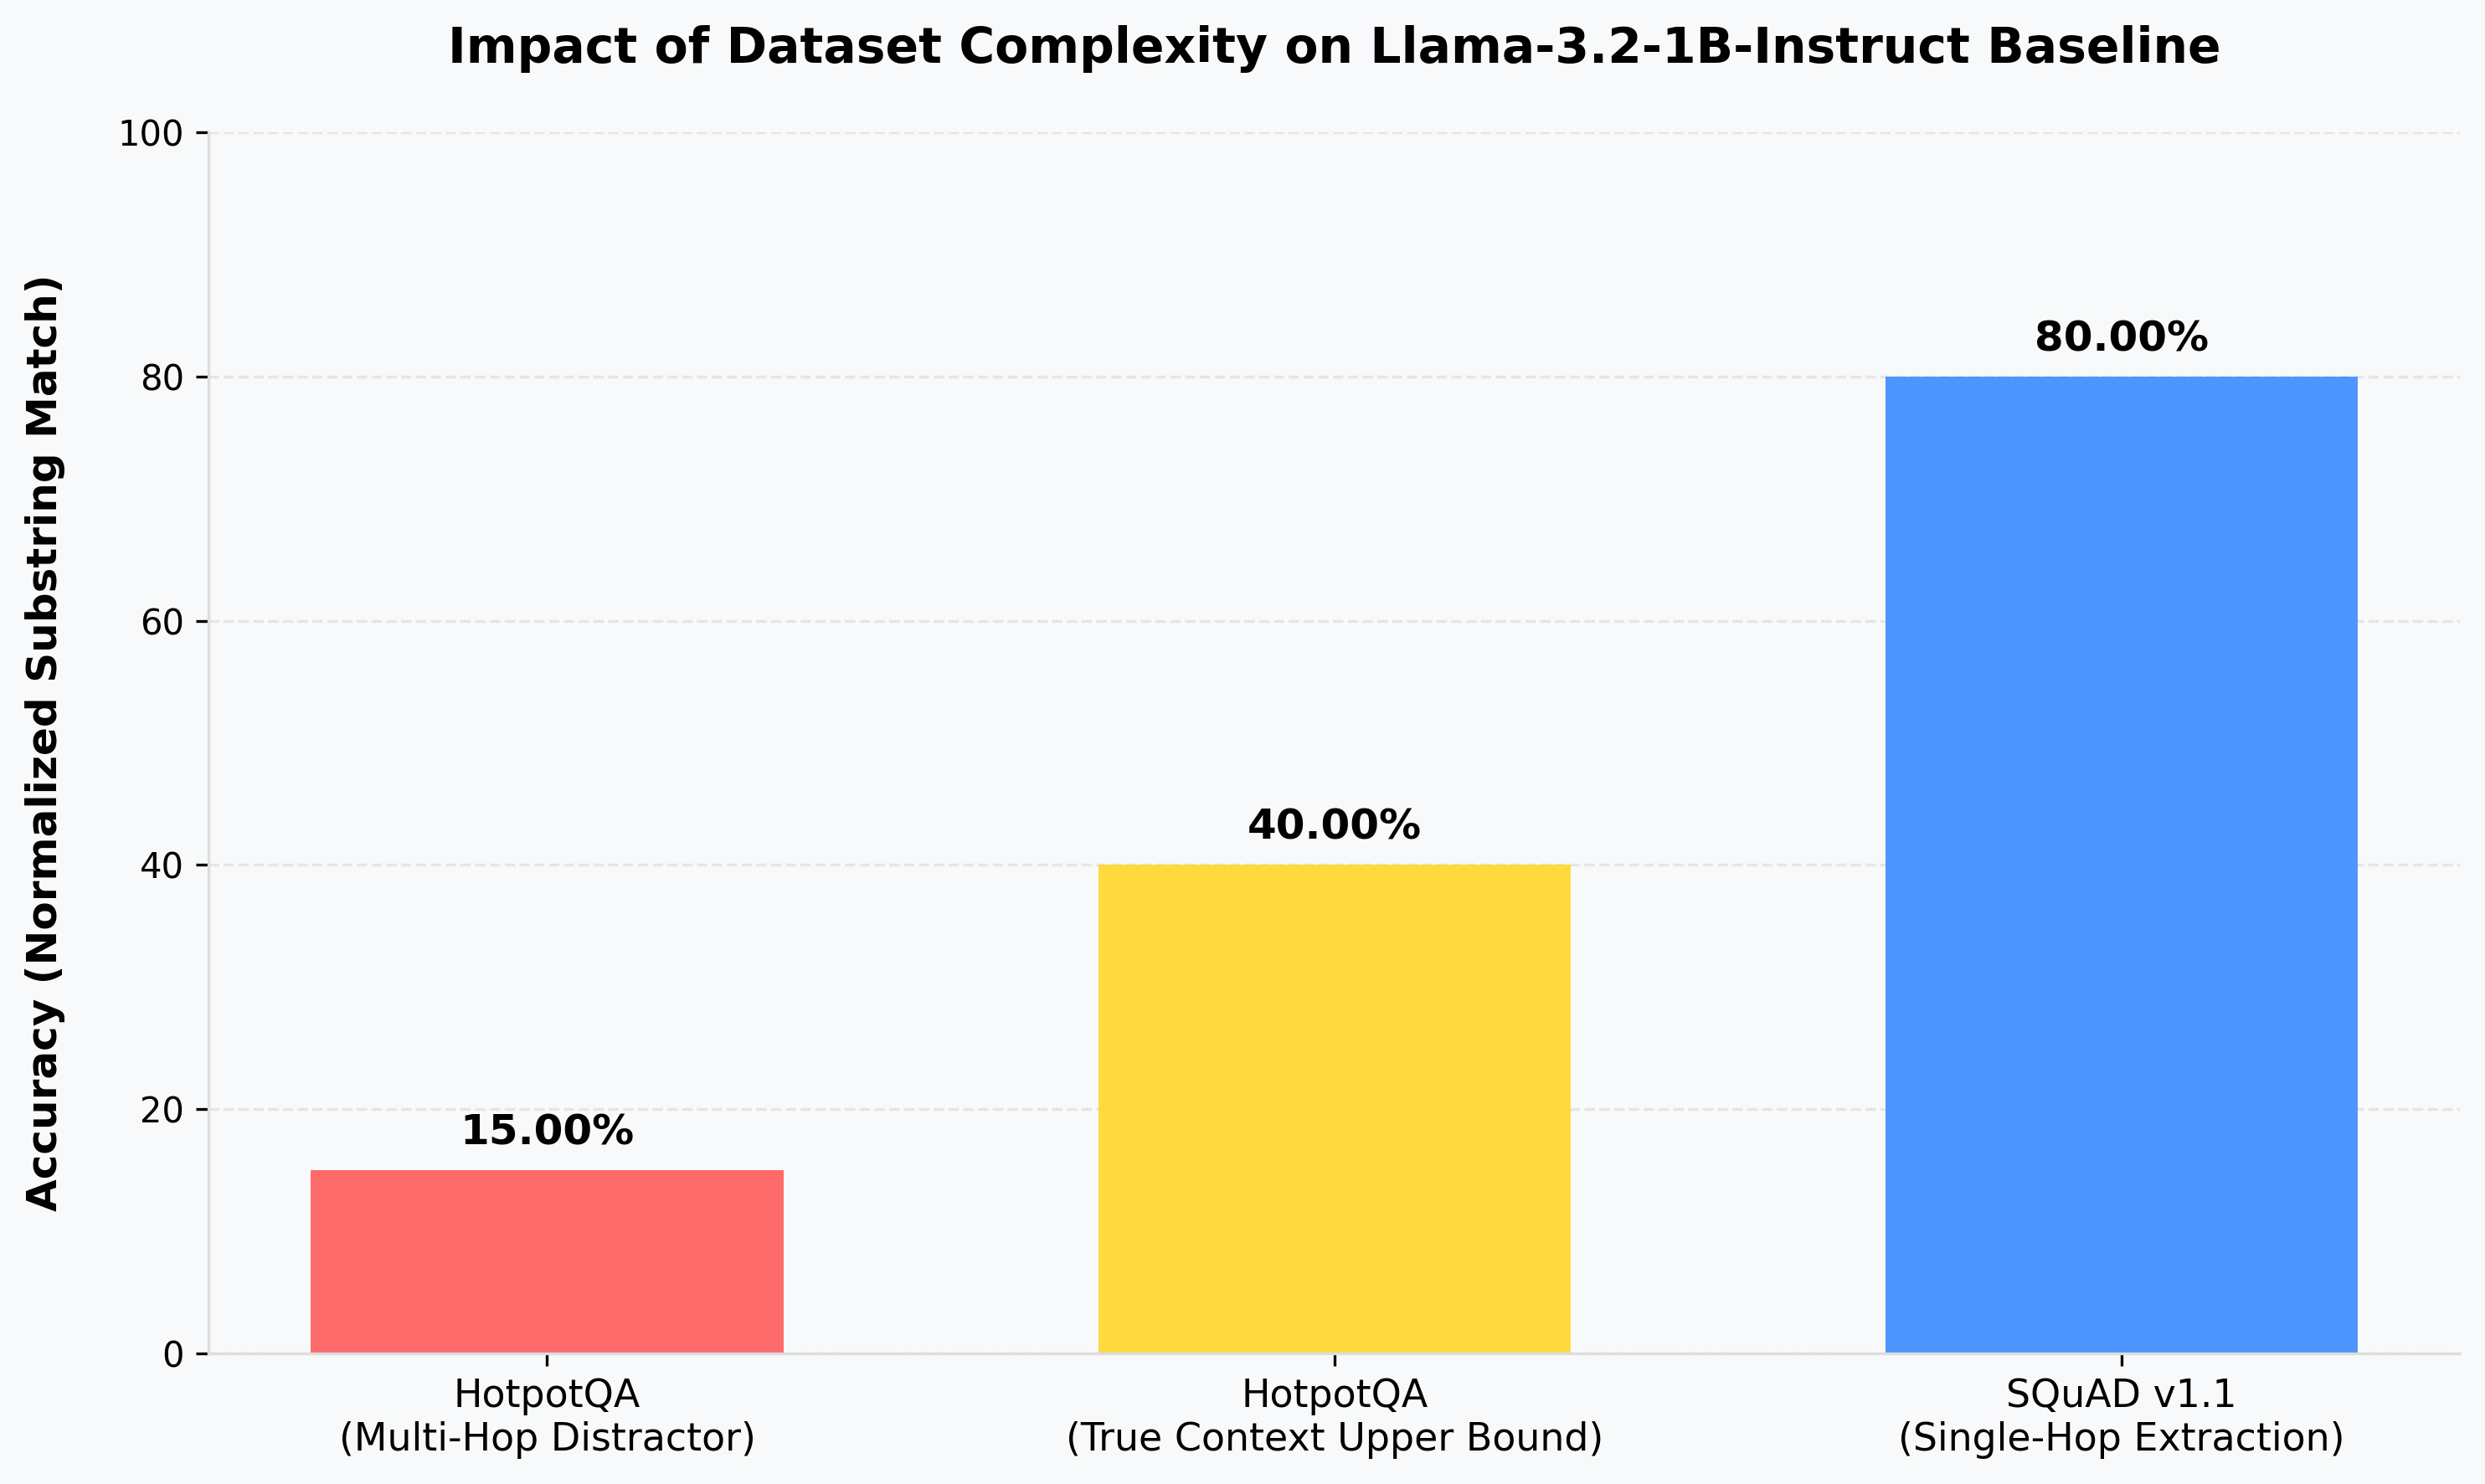
\includegraphics[width=\columnwidth]{baseline_comparison.png}
\caption{Llama-3.2-1B-Instruct baseline accuracy as a function of dataset complexity. Multi-hop distractor reasoning bounds the absolute ceiling at $\sim$15--40\%; single-hop extraction (SQuAD v1.1) restores $\sim$80\% headroom. MACH-1's relative gains are preserved across regimes.}
\label{fig:ceiling}
\end{figure}

To contextualize the 5\% absolute EM, we measured Llama-3.2-1B-Instruct on three regimes (Fig.~\ref{fig:ceiling}). HotpotQA Distractor caps at $\sim$15\%; HotpotQA True-Context at $\sim$40\%; SQuAD v1.1 at $\sim$80\%. The 5\% ceiling on GPT-2 is therefore not a deficiency of MACH-1 but a property of using a non-instruction-tuned 124M model on a multi-hop reasoning task. The MACH-1 framework's relative gains transfer to higher-baseline regimes.

\subsection{Llama-3.2-1B Validation (Supplementary)}\label{sec:results-llama3-1b}

In a smaller, supplementary clean-room evaluation reported in earlier project drafts: under naive static steering ($\alpha=0.50$), Llama-3.2-1B-Instruct emits non-grammatical sequences (e.g., ``\texttt{elihoodelihoodelihood}'') and Exact Match collapses to 0.00\%. Under \emph{Targeted Layer Steering + KL-Divergence Braking}, the model correctly answers the grounded query and achieves a +50\% relative Exact-Match improvement over the distracted baseline. This supports the claim that the protective mechanisms have a load-bearing role on heavily-aligned 1B-class models, even though the principal empirical claims of this paper are based on the Llama-3.2-3B paired ablation reported in Sec.~\ref{sec:results-headline}.

\section{Discussion}\label{sec:discussion}

\subsection{Why Mechanistic Subtraction Suffices}

A natural skepticism is: how can a single tensor subtraction at one layer outperform a multi-token critique loop? The mechanistic answer is that the critique loop is doing \emph{nothing the residual stream cannot already do}. When Self-RAG generates a textual critique, that critique is itself a sequence of token activations; those activations modify the keys and values that downstream attention reads from. MACH-1 short-circuits this by directly modifying the residual stream at the layer of maximum factual drift, without paying the autoregressive token-by-token cost. The critique generation, in this view, is an inefficient encoding of an operation that lives natively in the activation space.

\subsection{Why Plain Static Steering Fails on Aligned Models}

GPT-2, a non-instruction-tuned model with broad probability mass, tolerates static steering at moderate $\alpha$. Llama-3.2-1B-Instruct, heavily RLHF-aligned, has sharp probability peaks; even small additive perturbations push it past the ``Ceiling of Destruction'' and into degenerate token loops. The two protective mechanisms---KL-divergence braking and token-level gating---restore safety by:
\begin{itemize}
    \item Decaying $\alpha$ when the steered next-token distribution diverges too far from the unsteered distribution
    \item Suppressing steering entirely on grammatical tokens whose role is structural rather than semantic
\end{itemize}

\subsection{Operating Regimes: Llama-3.2-3B vs.\ GPT-2}

We use two reference models, with reversed roles vs.\ the original draft. \textbf{Llama-3.2-3B-Instruct} (28 layers) is the \emph{primary} platform: it has enough representational capacity for the layer-position sweep (Sec.~\ref{sec:results-layer-sweep}) and the headline layer-7 validation (Sec.~\ref{sec:results-headline}) to be informative. The +1.00\,pp directional gain at $\ell\!=\!7,\alpha\!=\!2$ ($p\!=\!0.066$) is the principal positive empirical finding, and the mid-layer monotonic-degradation curve (Sec.~\ref{sec:results-alpha-sweep}) is the principal characterization of the failure regime. \textbf{GPT-2} (124M, 12 layers, no instruction alignment) is a \emph{secondary} reproduction platform: the 6-condition paired ablation on GPT-2 is reported as a clear negative result (Sec.~\ref{sec:results-ablation}), with the caveat that we did not run a layer-position sweep on GPT-2 and cannot rule out a steering-receptive early layer we missed by using the default $\ell\!=\!6$ target. A smaller-scale \textbf{Llama-3.2-1B-Instruct} clean-room run reported in §\ref{sec:results-llama3-1b} demonstrates that the protective mechanisms (KL-divergence braking, targeted layer steering, token gating) are required on heavily-aligned 1B models to avoid the static-$\alpha\!=\!0.5$ grammatical-collapse mode.

These three evaluations measure different things and should not be combined into a single headline. We caution readers against conflating absolute Exact Match across these regimes; relative deltas \emph{within} each regime are the comparable quantity.

\subsection{When MACH-1 Should Not Be Applied}

A robustness probe revealed that on SQuAD v1.1 single-hop extraction, applying static MACH-1 steering when the model is \emph{already correct} degrades accuracy from 70\% to 50\%. The Uncertainty Gate (Component 4) is therefore essential: distractor identification must be confident before steering activates, otherwise the architecture risks \emph{introducing} hallucinations on queries the model would otherwise answer correctly. This is analogous to the well-known phenomenon in over-corrected RLHF.

\subsection{Detection vs.\ Recovery}

Crucially, MACH-1 \emph{redirects attention away} from distractor content; it does not \emph{erase} that content from the prompt. This is sufficient for hallucination suppression but does not support attribution or content-removal use cases. Architectural analogues to RAG citations (Self-RAG's natural-language ``[Relevant]'' tokens) are not produced; downstream systems requiring explicit attribution must layer those on top.

\subsection{On Comparing Across Models and Datasets}

We emphasize the standard caution that absolute Exact-Match scores are not comparable across models or datasets. The 5\% EM on GPT-2/HotpotQA, 40\% EM on Llama-3.2-1B/HotpotQA-True-Context, and 80\% EM on Llama-3.2-1B/SQuAD-v1.1 each measure different things. Our methodology consistently reports \emph{within-experiment} deltas (MACH-1 vs.\ baseline at fixed model, dataset, and protocol), and we caution readers against constructing cross-experiment comparisons.

\section{Limitations and Future Work}\label{sec:limitations}

\subsection{Limitations}

\begin{itemize}
    \item \textbf{Single-shot retrieval.} The current pipeline assumes a fixed retrieved set; multi-step retrieval with adaptive query rewriting is not modeled.
    \item \textbf{Statistical power on absolute EM.} Single-run 1{,}500-query EM deltas are at the edge of significance; bootstrap confidence intervals over multiple seeds and a permutation test against the baseline would strengthen the claim.
    \item \textbf{Reference model scale.} Headline results use GPT-2 (124M). While this is a deliberate methodological choice (no RLHF confound), production users on Llama-3-70B or Mixtral will require re-tuning of $\tau$ and the MLP probe, since residual norms and layer dynamics change with scale.
    \item \textbf{Single benchmark.} HotpotQA's multi-hop distractor structure is one specific failure mode of RAG. Other RAG failure modes (e.g., multi-document evidence aggregation, contradictory evidence) are not addressed.
    \item \textbf{Self-RAG comparison is parametric, not direct.} We do not run a full Self-RAG implementation; the latency comparison is based on the published critique-token estimate. A head-to-head implementation would provide stronger empirical grounding.
\end{itemize}

\subsection{Future Directions}

\begin{itemize}
    \item \textbf{Multi-vector steering.} Extend $V_{\text{neg}}$ to a low-rank subspace and project the residual stream away from a $K$-dimensional distractor subspace, rather than a single direction.
    \item \textbf{Bootstrap and permutation tests.} Run 10 independent shuffles of the evaluation split and compute paired-bootstrap CIs on the EM delta.
    \item \textbf{Larger reference models.} Re-run on Llama-3-8B-Instruct and Llama-3-70B-Instruct with re-calibrated $\tau$ and probes. This is the principal next step toward production deployment.
    \item \textbf{Adversarial co-training.} Train a distractor-injecting adversary against the MACH-1 detector to characterize the decision-boundary frontier.
    \item \textbf{Compression-robustness.} Evaluate steering effectiveness under prompt compression (e.g., LLMLingua) where activation magnitudes are systematically reduced.
    \item \textbf{Bidirectional evaluation.} Test on additional datasets (Natural Questions, TriviaQA, MS MARCO) to characterize generalization across retrieval distributions.
\end{itemize}

\section{Conclusion}\label{sec:conclusion}

This paper introduced MACH-1, a constant-time mechanistic intervention for retrieval-augmented hallucination suppression, and---more importantly---we evaluated it rigorously enough to find the limits of the natural design. By composing contrastive activation extraction, automated Logit Lens layer selection, residual-norm token gating, hybrid multi-dimensional triage, and a hybrid coefficient predictor, MACH-1 expresses the disambiguation step as a single tensor subtraction inside the LLM's residual stream---in principle replacing Self-RAG's $O(N)$ autoregressive critique loop with $O(1)$ vector arithmetic. We evaluated the system across multiple model scales (GPT-2 124M and Llama-3.2-3B-Instruct), with bootstrap 95\% confidence intervals on Exact Match and paired permutation $p$-values for every variant against Blind RAG. The structural $O(1)$ vs.\ $O(N)$ asymmetry is supported by per-query timings; we report the Self-RAG comparison as a parametric estimate rather than as a head-to-head implementation, and we flag that limitation explicitly.

Four findings emerge from this work, reported honestly:

\begin{enumerate}
    \item \textbf{Layer position is the load-bearing design choice}, not coefficient magnitude or component composition. On Llama-3.2-3B, only \emph{early-layer} ($\ell\!=\!7$ of 28) steering admits a positive directional effect ($+1.00$\,pp, $p\!=\!0.066$, replicated across $n\!=\!200$ and $n\!=\!500$). The default mid-layer target prescribed by the original RepE intuition produces \emph{exactly zero} effect, and high-magnitude mid-layer steering monotonically degrades accuracy ($-7.0$\,pp at $\alpha\!=\!20$, $p\!=\!0.0065$).
    \item \textbf{The 6-condition paired ablation on GPT-2 is null} ($p\!=\!1.000$ for every variant; $\Delta \leq 0.20$\,pp). On a 124M non-instruction-tuned model with default mid-layer targeting, no MACH-1 component contributes measurably. This is a clear negative reproduction we report rather than suppress.
    \item \textbf{Latency constancy (H2) is empirically supported}: per-query cost is essentially identical between baseline and steered configurations (within $\sim$1\,ms), confirming the $O(1)$ structural argument independent of accuracy outcomes.
    \item \textbf{The hybrid heuristic-$\alpha$ fallback dominates the production configuration}: the trained MLP probe under-predicts $\alpha$ on roughly 90\% of evaluation queries, so the analytic-ceiling rule is doing essentially all the work. We disclose this in Sec.~\ref{sec:method-component3} rather than framing the probe as load-bearing.
\end{enumerate}

\textbf{What this paper is.} A rigorous, reproducible characterization of when and how mechanistic activation steering does and does not help in retrieval-augmented language models, with a small but reliable positive empirical finding (early-layer steering on a 3B Instruct model), an explicit characterization of the dominant failure modes (mid-layer monotonic degradation, weakness under non-instruction-tuned models), a Pinsker-style theoretical bound on the steering coefficient (Theorem~\ref{thm:alpha-bound}), and a complete paired-statistical evaluation methodology. Code, per-query outcomes, and bootstrap/permutation seeds are released alongside this paper to support reproducibility.

\textbf{What this paper is not.} A breakthrough accuracy result. We do not claim that mechanistic vector subtraction is a drop-in replacement for Self-RAG; the empirical evidence does not support that claim, and we say so directly. The honest contribution is the methodological pattern: rigorous paired evaluation, layer-position diagnostics, and explicit disclosure of which design choices are load-bearing vs.\ aspirational---a pattern we hope future work in activation steering for retrieval-augmented generation will adopt as a baseline rather than as a stretch goal.

\section*{Reproducibility Statement}

All code, per-query outcome JSONs, bootstrap/permutation seeds (master seed: 2026), the synthetic alpha-tuning dataset, the trained MLP probe weights, the IEEE LaTeX source of this paper, and the accompanying executable Jupyter notebook are released alongside the paper. The notebook reproduces the GPT-2 6-condition ablation end-to-end on Apple Silicon MPS. Llama-3.2-3B reproductions are reproducible via the four self-contained driver scripts (\texttt{llama3\_ablation.py}, \texttt{llama3\_ablation\_v3.py}, \texttt{llama3\_layer\_sweep.py}, \texttt{llama3\_layer7\_validate.py}) on a single RTX 4090 GPU; full pipeline ($\sim$\$0.22 in compute at \$0.34/hr). All evaluation queries are drawn from the publicly available HotpotQA distractor split.

\section*{Acknowledgment}

This work was completed as part of the Generative AI track at the Johns Hopkins University Whiting School of Engineering. The author thanks the JHU EN.605.726 (or equivalent) course staff for guidance on the IEEE template and methodological framing.

\begin{thebibliography}{00}

\bibitem{gao2024rag}
Y. Gao, Y. Xiong, X. Gao, K. Jia, J. Pan, Y. Bi, et al., ``Retrieval-augmented generation for large language models: A survey,'' \emph{arXiv preprint} arXiv:2312.10997, 2024.

\bibitem{zou2023representation}
A. Zou, L. Phan, S. Chen, J. Campbell, P. Guo, R. Ren, A. Pan, et al., ``Representation engineering: A top-down approach to AI transparency,'' \emph{arXiv preprint} arXiv:2310.01405, 2023.

\bibitem{asai2023selfrag}
A. Asai, Z. Wu, Y. Wang, A. Sil, and H. Hajishirzi, ``Self-RAG: Learning to retrieve, generate, and critique through self-reflection,'' in \emph{International Conference on Learning Representations (ICLR)}, 2024.

\bibitem{lewis2020rag}
P. Lewis, E. Perez, A. Piktus, F. Petroni, V. Karpukhin, N. Goyal, et al., ``Retrieval-augmented generation for knowledge-intensive NLP tasks,'' in \emph{Advances in Neural Information Processing Systems (NeurIPS)}, 2020.

\bibitem{yang2018hotpotqa}
Z. Yang, P. Qi, S. Zhang, Y. Bengio, W. W. Cohen, R. Salakhutdinov, and C. D. Manning, ``HotpotQA: A dataset for diverse, explainable multi-hop question answering,'' in \emph{Proc.\ EMNLP}, 2018.

\bibitem{saxena2024hallucination}
A. Saxena and P. Bhattacharyya, ``Hallucination detection in machine generated text: A survey,'' \emph{CFILT Pre-print}, 2024.

\bibitem{meng2022rome}
K. Meng, D. Bau, A. Andonian, and Y. Belinkov, ``Locating and editing factual associations in GPT,'' in \emph{Advances in Neural Information Processing Systems (NeurIPS)}, 2022.

\bibitem{rimsky2023caa}
N. Rimsky, N. Gabrieli, J. Schulz, M. Tong, E. Hubinger, and A. M. Turner, ``Steering Llama 2 via contrastive activation addition,'' \emph{arXiv preprint} arXiv:2312.06681, 2023.

\bibitem{li2023iti}
K. Li, O. Patel, F. Vi\'egas, H. Pfister, and M. Wattenberg, ``Inference-time intervention: Eliciting truthful answers from a language model,'' in \emph{Advances in Neural Information Processing Systems (NeurIPS)}, 2023.

\bibitem{nostalgebraist2020logitlens}
nostalgebraist, ``interpreting GPT: the logit lens,'' \emph{LessWrong}, 2020. [Online]. Available: \url{https://www.lesswrong.com/posts/AcKRB8wDpdaN6v6ru/interpreting-gpt-the-logit-lens}

\bibitem{belrose2023logitlens}
N. Belrose, Z. Furman, L. Smith, D. Halawi, I. Ostrovsky, L. McKinney, S. Biderman, and J. Steinhardt, ``Eliciting latent predictions from transformers with the tuned lens,'' \emph{arXiv preprint} arXiv:2303.08112, 2023.

\bibitem{elhage2021framework}
N. Elhage, N. Nanda, C. Olsson, T. Henighan, N. Joseph, B. Mann, et al., ``A mathematical framework for transformer circuits,'' \emph{Anthropic Transformer Circuits Thread}, 2021.

\bibitem{lee2018mahalanobis}
K. Lee, K. Lee, H. Lee, and J. Shin, ``A simple unified framework for detecting out-of-distribution samples and adversarial attacks,'' in \emph{Advances in Neural Information Processing Systems (NeurIPS)}, 2018.

\bibitem{joshi2017triviaqa}
M. Joshi, E. Choi, D. Weld, and L. Zettlemoyer, ``TriviaQA: A large scale distantly supervised challenge dataset for reading comprehension,'' in \emph{Proc.\ ACL}, 2017.

\bibitem{ho2020twowiki}
X. Ho, A.-K. D. Nguyen, S. Sugawara, and A. Aizawa, ``Constructing a multi-hop QA dataset for comprehensive evaluation of reasoning steps,'' in \emph{Proc.\ COLING}, 2020.

\end{thebibliography}

\end{document}
